
\documentclass{beamer} 


\mode<presentation>
{
  \usetheme[hideothersubsections]{Boadilla}
  % or ...

  \setbeamercovered{transparent}
  % or whatever (possibly just delete it)
}

\usepackage{tikz}
\usepackage{graphicx}
\usepackage[english]{babel}
\usepackage{tikz}
\usetikzlibrary{decorations.pathreplacing,angles,quotes}
\usetikzlibrary{shapes, shadows, arrows, positioning,fit}
\usepackage{multirow, booktabs, adjustbox}
\usepackage{relsize, lscape}
\usepackage[utf8]{inputenc}
\usepackage{adjustbox}
\usepackage{verbatim}
\usepackage{listings, amsmath}
\usepackage{natbib}
\usepackage{tcolorbox}
\usepackage{transparent}
\usepackage{comment}


\usepackage{relsize, lscape}
\usepackage{multirow, booktabs, adjustbox}
\usepackage{lipsum} % Used for inserting dummy 'Lorem ipsum' text into the template
\usepackage{array}
\usepackage{graphicx}
\usepackage{hyperref}
\usepackage{multicol}


% or whatever

\usepackage{times}
\usepackage[T1]{fontenc}
% Or whatever. Note that the encoding and the font should match. If T1
% does not look nice, try deleting the line with the fontenc.


\newcommand{\nit}[1]{\textrm{\textit{{\color{red}[#1]}}}}
\newcommand{\highlight}[1]{\colorbox{yellow}{$\displaystyle #1$}}
\newcommand{\highlightw}[1]{\colorbox{white}{$\displaystyle #1$}}
\newcommand{\highlightr}[1]{\colorbox{red}{$\displaystyle #1$}}
\newcommand{\tabitem}{~~\llap{\textbullet}~~}


\def\gray{\color{lightgray}}
\def\red{\color{red}}
\def\white{\color{white}}
\def\brown{\color{brown}}
\def\black{\color{black}}
\def\blue{\color{blue}}

\beamertemplatenavigationsymbolsempty

\renewcommand{\topfraction}{0.9}
\newsavebox{\codebox}
\lstset{
basicstyle=\scriptsize\tt,
}

\newcolumntype{P}[1]{>{\raggedright\arraybackslash}p{#1}}

\newcommand{\backupbegin}{
   \newcounter{finalframe}
   \setcounter{finalframe}{\value{framenumber}}
}
\newcommand{\backupend}{
   \setcounter{framenumber}{\value{finalframe}}
}

\newcommand\Wider[2][3em]{%
\makebox[\linewidth][c]{%
  \begin{minipage}{\dimexpr\textwidth+#1\relax}
  \raggedright#2
  \end{minipage}%
  }%
}
%control cross slide button format
\setbeamertemplate{button}{\tikz
  \node[
  inner xsep=2pt,
  draw=structure!50,
  fill=structure!50,
  rounded corners=2pt]  {\Large\insertbuttontext};}


\subject{Research Transparency}
% This is only inserted into the PDF information catalog. Can be left
% out. 

% If you have a file called "university-logo-filename.xxx", where xxx
% is a graphic format that can be processed by latex or pdflatex,
% resp., then you can add a logo as follows:

% \pgfdeclareimage[height=0.5cm]{university-logo}{university-logo-filename}
% \logo{\pgfuseimage{university-logo}}



% Delete this, if you do not want the table of contents to pop up at
% the beginning of each subsection:
%\AtBeginSubsection[]
%{
%  \begin{frame}<beamer>{Outline}
%    \tableofcontents[currentsection,currentsubsection]
%  \end{frame}
%}


% If you wish to uncover everything in a step-wise fashion, uncomment
% the following command: 

\beamerdefaultoverlayspecification{<.->}


\begin{document}

\title[] % (optional, use only with long paper titles)
{Open Policy Analysis: Principles and Applications}

\subtitle
{}

\author[] % (optional, use only with lots of authors)
{Fernando~Hoces de la Guardia}
% - Give the names in the same order as the appear in the paper.
% - Use the \inst{?} command only if the authors have different
%   affiliation.

\institute[] % (optional, but mostly needed)
{%
  UC Berkeley:\\
  Berkeley Initiative for Transparency in the Social Sciences\\
}
% - Use the \inst command only if there are several affiliations.
% - Keep it simple, no one is interested in your street address.

\date[] % (optional, should be abbreviation of conference name)
{GiveWell\\
August 23rd, 2018}



\begin{frame}
  \titlepage
\end{frame}


\setbeamercovered{invisible}

\begin{frame}{Motivation: To Producers of Policy Analysis}
\vspace{-0.5in}
\begin{align*}
\intertext{Cynical view:}
\text{Policy Analysis} &= \text{Research} - \text{Novelty} - \text{Rigor}  
\onslide<2->{\intertext{Optimists view:}
\text{Policy Analysis} &= \text{Research} - \text{Novelty}  + \text{Relevance}  - \text{Rigor} }
\onslide<3>{\intertext{Our proposal:}
\text{Open Policy Analysis} &= \text{Research} - \text{Novelty}+ \text{Relevance}    }
\end{align*}

\end{frame}

\begin{frame}{Motivation: To Producers of Policy Analysis}
\vspace{-0.5in}
\begin{align*}
\intertext{Cynical view:}
\text{Policy Analysis} &= \text{Research} - \text{Novelty} - \text{Rigor}  
\onslide<2->{\intertext{Optimists view:}
\text{Policy Analysis} &= \text{Research} - \text{Novelty}  + \text{Relevance}  - \text{Rigor} }
\onslide<3>{\intertext{Our proposal:}
\text{Open Policy Analysis} &= \text{Research} - \text{Novelty}+ \text{Relevance}    }
\end{align*}

\end{frame}


\begin{frame}{Motivation: To Producers of Research}
Think for a second of the one paper that you are most proud of. 
Now think of the best estimate that you have in that paper. 
\bigskip
\pause
\begin{itemize}
\item Do you know if that paper had any \textbf{direct} effect on public policy?
(direct: estimate used in policy report, law, testimony\\
indirect: general knowledge, NYT op-ed)
\pause
\item If that estimate where to be revise to by a factor of 2 (or 10). How should the policy analysis change? 
\end{itemize}
\end{frame}

\setbeamercovered{transparent}

\part{Paper 1}


\title[Open Policy Analysis ] % (optional, use only with long paper titles)
{Why We Need Open Policy Analysis}

\subtitle
{}

\author[] % (optional, use only with lots of authors)
{Fernando~Hoces de la Guardia\inst{1}\\
Sean~Grant\inst{2}\\
Edward Miguel\inst{1}}
% - Give the names in the same order as the appear in the paper.
% - Use the \inst{?} command only if the authors have different
%   affiliation.

\institute[] % (optional, but mostly needed)
{
  \inst{1}%
  UC Berkeley:\\
  Berkeley Initiative for Transparency in the Social Sciences\\
  \inst{2}%
  RAND\\
}
% - Use the \inst command only if there are several affiliations.
% - Keep it simple, no one is interested in your street address.

\date[] % (optional, should be abbreviation of conference name)
{GiveWell\\
August 23rd, 2018}


% - Either use conference name or its abbreviation.
% - Not really informative to the audience, more for people (including
%   yourself) who are reading the slides online

\begin{frame}
  \titlepage
\end{frame}




% Structuring a talk is a difficult task and the following structure
% may not be suitable. Here are some rules that apply for this
% solution: 

% - Exactly two or three sections (other than the summary).
% - At *most* three subsections per section.
% - Talk about 30s to 2min per frame. So there should be between about
%   15 and 30 frames, all told.

% - A conference audience is likely to know very little of what you
%   are going to talk about. So *simplify*!
% - In a 20min talk, getting the main ideas across is hard
%   enough. Leave out details, even if it means being less precise than
%   you think necessary.
% - If you omit details that are vital to the proof/implementation,
%   just say so once. Everybody will be happy with that.
%%%%%%%%%%%%%%%%%%%%%%%%%%%%%%%%%%%%%%%%%%%%%%%%%%%%%%%%%%%%%%%%%%%%%%%
%%%%%%%%%%%%%%%%%%%%%%%%%%%%%%%%%%%%%%%%%%%%%%%%%%%%%%%%%%%%%%%%%%%%%
 
\section[Evidence Based]{Policy Analysis And The Evidence-Based Policy Movement}

\begin{frame}{Policy Analysis And The Evidence-Based Policy Movement}
Evidence-Based movement is growing. 
\begin{itemize}
\item ``The golden age of evidence-based policy'' (Haskins 2017).
%\begin{itemize}
\item Credible causal evidence (Angrist \& Pischke, 2010)
\item Transparency and reproducibility of research (Miguel et al. 2014).
%\end{itemize} 
\item Commission on Evidence-Based Policymaking (CEBP, 2017)
\end{itemize}
\pause
Policy Analysis is a fundamental link. 
\begin{itemize}
\item As many definitions as textbooks (Dunn, 2015; Weimer \& Vining, 2017; Williams, 1971)
\item Common denominator: client-oriented empirical analysis meant to inform a specific policy debate
\item Aspires at scientific rigor. (Wildavsky 1979),
\end{itemize}
\end{frame} 


\begin{frame}{One Ideal Evidence-Based Policy Link}

\tikzstyle{agent} = [diamond, draw, node distance= 7em, minimum height=5em, minimum width=5em]
\tikzstyle{line} = [draw, -stealth]

\tikzstyle{line_enph} = [draw, red, ultra thick]
\tikzstyle{inp} = [draw, circle, text centered, minimum height=2em, text width=2em, node distance= 10em]
\tikzstyle{outp} = [draw, circle, text centered, minimum height=2em, text width=2em, node distance= 10em]
\tikzstyle{block1} = [draw, circle,  text width=5em, text centered, minimum height=7em, node distance= 5em]
\tikzstyle{block2} = [draw, circle,  text width=7em, text centered, minimum height=2em, node distance= 5em]
\tikzstyle{block3} = [draw, rounded rectangle,  text width=5em, text centered, minimum height=2em, node distance= 5em]


\begin{figure}[h!]\centering

\begin{tikzpicture}[thick,scale=0.6, every node/.style={scale=0.6}]

%% The oddly shaped truth
\node[regular polygon, regular polygon sides=3,
              draw, fill=white,
              inner sep=.1em,
              shape border rotate=70](tru){Truth};


%%%%%Researcher 1 and Inputs: depends on R_1%%%%%%%
\node [block1, right = 2em of tru](R_1){Research\linebreak $(R)$};
\node [block1,inner sep=0em, right = 2em of R_1](PA_1){Policy \linebreak Analysis: ($PA$) \linebreak  Gains  \& \linebreak losses};
\node [block1, above right = 0em and 8em of R_1](PM_1){Policy\linebreak Maker 1};
\node [block1, below right = 0em and 8em of R_1](PM_2){Policy\linebreak Maker 2};

\node [block3, right = 2em of PM_1](PC_1){Support};
\node [block3, right = 2em of PM_2](PC_2){Oppose};


%%%%% Draw edges col 2%%%%%%%%%%%%%%%%%
%Research  to PA
\draw [line](tru) -- (R_1);
\draw [line](R_1) -- (PA_1);
%PA to PM
\draw [line](PA_1) -- (PM_1);
\draw [line](PA_1) -- (PM_2);
%PM to PC
\draw [line](PM_1) -- (PC_1);
\draw [line](PM_2) -- (PC_2);

%%%%%%%%%%%%%%%%%%%%%%%%%%%%%%%%%%%%%%



\draw[decoration={brace}, decorate] (6.2,3.4) -- node[above=6pt](lab4){{\Large Observed by citizens} }(15.2,3.4);




\end{tikzpicture}
\vspace{-.8em}
\end{figure}
\end{frame}


\section[Crisis in Research]{Reproducibility Crisis In Empirical Research}

\begin{frame}{Reproducibility Crisis In Empirical Research}

\begin{itemize}
%\item  Researchers believe in good science but don't practices it (Anderson, Martinson, \& De Vries 2007).  
%\pause
%\item ``Most published research is false'' Ioannidis (2005). 
\item Large magnitude of publication bias (Franco et al 2014).  
\item Evidence of extensive p-hacking across social science disciplines (Gerber et al 2008, Brodeur et al 2016).
\item Replication rates are low (Collaboration et al, 2015 , Camerer et al, 2016). 
\item Computational reproducibility is also low (Stodden et al 2016, Chang and Li 2015, Gertler et al 2018).
\end{itemize}

\end{frame} 


\section[Crisis in PA]{Credibility Crisis Of Policy Analysis}

\begin{frame}{Credibility Crisis Of Policy Analysis}
\begin{itemize}
\item Incredible Certitudes  (Manski, 2013) 
\item Report wars (Wesselink et al, 2013) 
\pause
\item Alternative facts (``The Death of Expertise'' Nichols, 2017; ``The Death of Truth'', Kakutani 2018; ``Truth Decay'', Rich \& Kavanagh 2018)
\end{itemize}
\end{frame} 

\begin{frame}[shrink=30]{How This Affects The Evidence Based Policy Link?}
\pause

\tikzstyle{agent} = [diamond, draw, node distance= 7em, minimum height=5em, minimum width=5em]
\tikzstyle{line} = [draw, -stealth]

\tikzstyle{line_d} = [draw, dashed, -stealth]
\tikzstyle{inp} = [draw, circle, text centered, minimum height=2em, text width=2em, node distance= 10em]
\tikzstyle{outp} = [draw, circle, text centered, minimum height=2em, text width=2em, node distance= 10em]
\tikzstyle{block1} = [draw, circle,  text width=3em, text centered, minimum height=2em, node distance= 5em]
\tikzstyle{block2} = [draw, circle,  text width=4em, text centered, minimum height=2em, node distance= 5em]
\tikzstyle{block3} = [draw, rounded rectangle,  text width=5em, text centered, minimum height=2em, node distance= 5em]

\begin{figure}[h!]
\centering
\hspace*{0.2\linewidth}
\begin{tikzpicture}[thick,scale=0.2, every node/.style={scale=0.8}]

%% The oddly shaped truth
\node[regular polygon, regular polygon sides=3,
              draw, fill=white,
              inner sep=.1em,
              shape border rotate=70](tru){Truth};


%%%%%Researcher 1 and Inputs: depends on R_1%%%%%%%
\node [block1, right = 5em of tru](R_2){$R_2$};
\node [block1, above = 8em of R_2](R_1){$R_1$} node [left = -0.1em of R_1, text width = 5em]{Large Treatment Effect};
\node [block1, below = 8em of R_2](R_3){$R_3$} node [left = -0.1em of R_3, text width = 5em]{Small Treatment Effect};

\draw[decoration={brace,mirror}, decorate] (13,-33) -- node[below=6pt, text width = 4.8em](lab1){Researchers Degrees of 
Freedom}(18,-33);

\draw[decoration={brace,mirror}, decorate] (29,-33) -- node[below=6pt, text width = 5em](lab2){Policy Analyst Degrees of 
Freedom}(34,-33);

\draw[decoration={brace}, decorate] (31,33) -- node[below=2pt]{Observed by citizens}(70,33);

%\node [agent](Researcher_1){$R_1$} node [left = 0.6em of Researcher_1, text width = 8em]{Large Treatment Effect};

\node [block1, right = 5em of R_1](PA_12){$PA_{1,2}$};
\node [block1, above = .5em of PA_12](PA_11){$PA_{1,1}$} node [right = -0.1em of PA_11, text width = 5em]{Large gains only};
\node [block1, below = .5em of PA_12](PA_13){$PA_{1,3}$};

\node [block1, right = 5em of R_2](PA_22){$PA_{22,}$};
\node [block1, above = .5em of PA_22](PA_21){$PA_{2,1}$};
\node [block1, below = .5em of PA_22](PA_23){$PA_{2,3}$};

\node [block1, right = 5em of R_3](PA_32){$PA_{3,2}$};
\node [block1, above = .5em of PA_32](PA_31){$PA_{3,1}$};
\node [block1, below = .5em of PA_32](PA_33){$PA_{3,3}$} node [right = -0.1em of PA_33, text width = 5em]{Large losses only};


\node [block2, above right = 3em and 15em of R_2](PM_1){Policy\linebreak Maker 1};
\node [block2, below right = 3em and 15em of R_2](PM_2){Policy\linebreak Maker 2};

\node [block3, right = 3em of PM_1](PC_1){Support};
\node [block3, right = 3em of PM_2](PC_2){Oppose};


%%%%% Draw edges col 2%%%%%%%%%%%%%%%%%
%Truth to research
\draw [line](tru) -- (R_1);
\draw [line_d](tru) -- (R_2);
\draw [line_d](tru) -- (R_3);


%Research  to PA
\draw [line_d](R_1) -- (PA_13);
\draw [line_d](R_1) -- (PA_11);
\draw [line](R_1) -- (PA_12);

\draw [line_d](R_2) -- (PA_23);
\draw [line_d](R_2) -- (PA_21);
\draw [line_d](R_2) -- (PA_22);

\draw [line_d](R_3) -- (PA_33);
\draw [line_d](R_3) -- (PA_31);
\draw [line_d](R_3) -- (PA_32);



%PA to PM
\draw [line](PA_11) -- (PM_1);
\draw [line](PA_33) -- (PM_2);
%PM to PC
\draw [line](PM_1) -- (PC_1);
\draw [line](PM_2) -- (PC_2);

%%%%%%%%%%%%%%%%%%%%%%%%%%%%%%%%%%%%%%




\end{tikzpicture}
\end{figure}
%\end{comment}
\end{frame}


\begin{comment}

\begin{frame}{}
\begin{table}[ht]
\centering
\begin{tabular}[t]{|l|c|c|}
\hline
& Empirical  & Policy \\
& Research & Analysis \\

\hline
Problems & Reproducibility  &  Credibility \\
				 &  Crisis & Crisis \\
\hline
Solutions & {\white  \textit{Open Science } }&    {\white \textit{Open Policy Analysis } }\\
 &   {\white Principles, Guidelines, } &   {\white Principles, Guidelines,}\\
 &  {\white  Applications} &   {\white Applications}\\

\hline
\end{tabular}
\end{table}%
\end{frame}


\begin{frame}[noframenumbering]{}
\begin{table}[ht]
\centering
\begin{tabular}[t]{|l|c|c|}
\hline
& Empirical  & Policy \\
& Research & Analysis \\

\hline
Problems & Reproducibility  &  Credibility \\
				 &  Crisis & Crisis \\
\hline
Solutions &  \textit{Open Science }&    {\white \textit{Open Policy Analysis } }\\
 &   Principles, Guidelines, &   {\white Principles, Guidelines,}\\
 &    Applications  &   {\white Applications}\\

\hline
\end{tabular}
\end{table}%
\end{frame}

\end{comment}

\begin{frame}{Relevance}
Main consequences of policy analysis that lacks openness:
\begin{enumerate}
\item Cherry picking evidence.
\item Challenging to automate and Improve systematically recurring reports.
\item Difficulty understanding how research informs policy analysis.
\end{enumerate}
\end{frame}

\begin{frame}{Cherry Picking Evidence}
\pause
\begin{exampleblock}{}
  {\large ``When I was director of the CBO, I was very frustrated when we would write a policy report [saying] a certain policy would have these two advantages and these two disadvantages, and the advocates would quote only the part about the advantages, and the opponents would quote only the part about the disadvantages. That encourages the view that there are simple answers. There aren't generally simple answers. There are trade-offs.''
%I would strayed from Josh Angrist.. what is the right word... [DC says] straight jacket (in a friendly tone). That is a %good one. Although if I were to have a hierarchy of what is the strongest, I would probably start wearing Josh's straight %jacket
}
  \vskip3mm
  \raggedleft{\small--- Douglas Elmendorf (Director of CBO, 2009-2015)} \footnotesize{ \linebreak  Harvard Magazine, 2016} 
  	  
\end{exampleblock}
\end{frame} 

%6mins



\begin{frame}{Difficulty Understanding how Research Informs Policy Analysis}
\begin{itemize}
\item What happens when new research emerges?
\begin{itemize}
\item What if $\hat{\tau}($ Blattman, Fiala, and Martinez 2020$) = \frac{1}{2}\hat{\tau}($ Blattman, Fiala, and Martinez 2013$)$? Or $\tau_{2020} = 2\tau_{2013}$?
\end{itemize}
\pause
\item Where a the largest unknowns in the policy analysis?
\begin{itemize}
\item GiveWell lists at least 100 parameters in its cost-effectiveness analysis. What are the 5/10 most important ones?
\end{itemize}
\pause
\item Where is the marginal piece of research most informative for this analysis?
\begin{itemize}
\item Are the gaps in knowledge for this PA guiding the research agenda?
\end{itemize}
\end{itemize}
\end{frame} 


\section[Solutions]{The Open Science Movement}

\begin{frame}{The Open Science Movement}

\begin{itemize}
\item Definition of principles of Open Science/Research Transparency (Miguel et al 2014)
\item Development of guidelines to operationalize principles of Open Science (Nosek et al 2015)
\item Journals and funders: Journals (Science + 5k other journals), Registries (AEA), Funders (NIH, NSF and multiple donors)
\end{itemize}

\end{frame} 


\begin{frame}{Open Science}
\begin{table}[ht]
\centering
\begin{tabular}[t]{|l|c|c|}
\hline
& Empirical  & Policy \\
& Research & Analysis \\

\hline
Problems & Reproducibility  &  Credibility \\
				 &  Crisis & Crisis \\
\hline
Solutions &  \textit{Open Science }&    {\white \textit{Open Policy Analysis } }\\
 & Principles, Guidelines,  &   {\white Principles, Guidelines,}\\
 & Applications &   {\white Applications}\\

\hline
\end{tabular}
\end{table}%
\end{frame}

\begin{frame}[noframenumbering]{Open Policy Analysis}
\begin{table}[ht]
\centering
\begin{tabular}[t]{|l|c|c|}
\hline
& Empirical  & Policy \\
& Research & Analysis \\

\hline
Problems & Reproducibility  &  Credibility \\
				 &  Crisis & Crisis \\
\hline
Solutions &  \textit{Open Science }&    \textit{Open Policy Analysis } \\
 & Principles, Guidelines,  &   Principles\\
 & Applications &   \\

\hline
\end{tabular}
\end{table}%
\end{frame}


\begin{frame}[shrink=25, label = pa_comp]{The Process of Policy Analysis}

\tikzstyle{estimate} = [diamond, draw, node distance= 7em,text width = 5em, minimum height=5em, minimum width=5em, align = center]
\tikzstyle{line} = [draw, -stealth]
\tikzstyle{line_enph} = [draw, red, ultra thick]
\tikzstyle{inp} = [draw, rectangle, text centered, minimum height=3em, text width=2em, node distance= 2em]
\tikzstyle{source} = [draw, rectangle, text centered, minimum height=8em, text width=5em, node distance= 10em]
\tikzstyle{model} = [draw, rectangle, text centered, minimum height=8em, text width=15em, node distance= 10em]
%\tikzstyle{outp} = [draw, ellipse, text centered, minimum height=2mm, text width=2em, node distance= 10em]
%\tikzstyle{block} = [draw, rectangle,  text width=8em, text centered, minimum height=55mm, node distance= 5em]


%\begin{adjustbox}{max totalsize={1\textwidth}{.8\textheight},center}

\begin{figure}[h!]\centering 
\hspace*{-2.5em}
\begin{tikzpicture}[thick,scale=0.6, every node/.style={scale=0.6}]
\setbeamercovered{invisible}

%%%%%Nodes: Sources%%%%%%%
\node [source](D_1){$Data$};
\node [source, below = 1em of D_1](Lit){$Research$};
\node [source, below = 1em of Lit](OR){\textit{Guess work}};


\draw[decoration={brace,mirror}, decorate] (-1.2,-10) -- node[below=6pt] {$Sources$}(1.1,-10);

\draw[decoration={brace,mirror}, decorate] (4.8,-11.3) -- node[below=6pt] {$Inputs$}(6.2,-11.3);


%node[below = 1em ](OR) -- node[below = 6em]{asd}(OR)


%\onslide<2-5>\node [source, color=red](Lit){$Research$};

%%%%%Nodes: Inputs%%%%%%%
\node [inp, above right = 1em and 6em of  D_1 ](I_1){$I_1$};
\node [inp, below = 1em of I_1](I_2){$I_2$};
\node [inp, below = 8em of I_2](I_j){$I_j$};
\node [inp, below right = 1em and 6em of OR ](I_last){$I_J$};




\path (I_2) -- node[auto=false, rotate=90, anchor=north, outer sep=-0.5em]{\ldots} (I_j);
\path (I_j) -- node[auto=false, rotate=90, anchor=north, outer sep=-0.5em]{\ldots} (I_last);

%%%%%Paths connecting Sources with Inputs%%%%%%%
\draw [line](D_1.east) -- (I_1.west);
\draw [line](D_1.east) -- (I_2.west);
\draw [line, opacity=1, anchor=center](Lit.east) -- (I_j.west);
\draw [line, opacity=1, anchor=center](OR.east) -- (I_last.west);


\draw [line, opacity=.3][xshift=1em](D_1.east) -- ([yshift=-8 em]I_1.west);
\draw [line, opacity=.3][xshift=1em](D_1.east) -- ([yshift=-10 em]I_1.west);

\draw [line, opacity=.3][xshift=1em](Lit.east) -- ([yshift=7 em]I_j.west);
\draw [line, opacity=.3][xshift=1em](Lit.east) -- ([yshift=-5 em]I_j.west);

\draw [line, opacity=.3][xshift=1em](OR.east) -- ([yshift=3 em]I_last.west);
\draw [line, opacity=.3][xshift=1em](OR.east) -- ([yshift=5 em]I_last.west);


%%%%%Node and paths for model%%%%%%%
\node [model, below right = 2em and 10em of D_1](model){$Model$};
\draw [line](I_1) -| (model);
\draw [line](I_2) -| (model);
\draw [line](I_j) |- (model);
\draw [line](I_last) -| (model);


%%%%%Node and paths for policy estimates%%%%%%%
\node [estimate, right = 5em of model](PE_2){$Policy$ $Estimate_2$};
\node [estimate, above = 5em of PE_2](PE_1){$Policy$ $Estimate_1$};
\node [estimate, below = 5em of PE_2](PE_3){$Policy$ $Estimate_3$};


\draw [line] (model.east) -- (PE_1.south west);
\draw [line] (model.east) -- (PE_2.west);
\draw [line] (model.east) -- (PE_3.north west);


\end{tikzpicture}
\end{figure}

\end{frame}

\begin{frame}{Principles for Open Policy Analysis}
Proposed principles:
\begin{enumerate}
\item Computational Reproducibility
\item Analytic Transparency
\item Output Transparency 
\end{enumerate}
\end{frame} 


\begin{frame}{Principle 1}
\begin{columns}
\begin{column}{0.3\textwidth}
\textbf{Computational Reproducibility}
\begin{itemize}
\item Literate \\ Programming
\item Version control
\item File structure
\item Label sources
\end{itemize}
\end{column}
\begin{column}{0.65\textwidth}  %%<--- here
    \begin{center}
     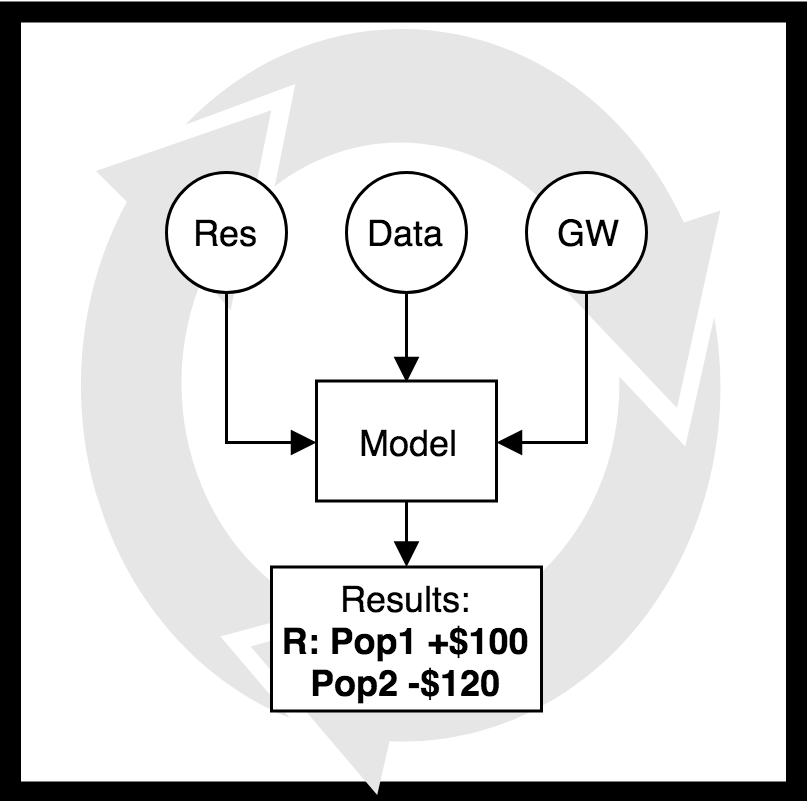
\includegraphics[width=1\textwidth]{../Images/repro.png}
     \end{center}
\end{column}
\end{columns}
\end{frame}

\begin{frame}{Principle 2}
\begin{columns}
\begin{column}{0.25\textwidth}
   \textbf{Analytic Transparency}
   \begin{itemize}
   \item Open code
   \item Open data
   \item  Report as Dynamic Document    
   \end{itemize}
\end{column}
\begin{column}{0.7\textwidth}  %%<--- here
    \begin{center}
     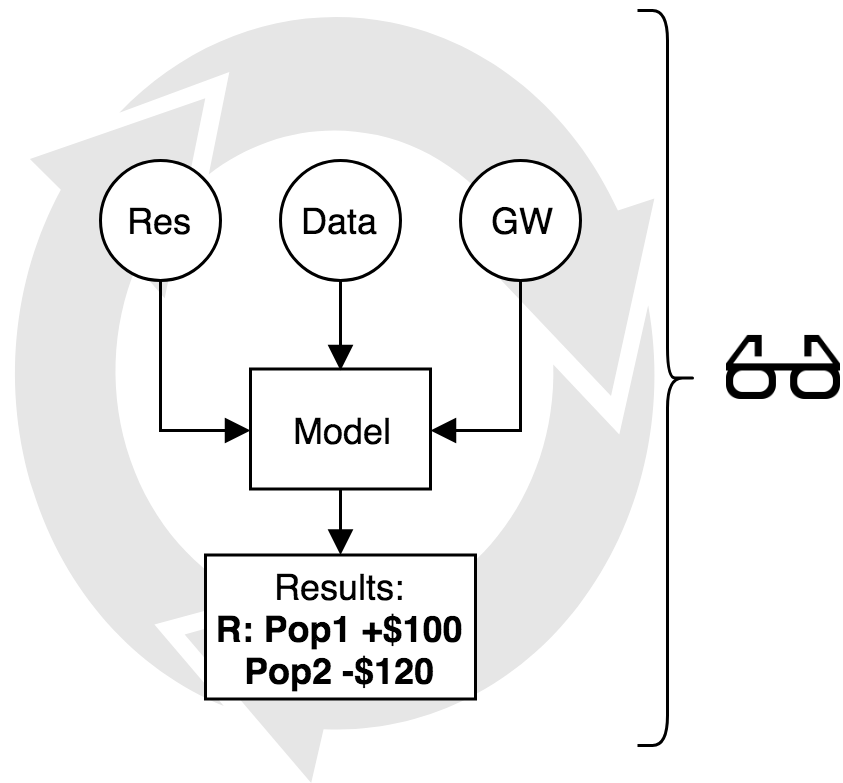
\includegraphics[width=1\textwidth]{../Images/a_transp.png}
     \end{center}
\end{column}
\end{columns}
\end{frame}

\begin{frame}{Principle 3}
\begin{columns}
\begin{column}{0.3\textwidth}
 \textbf{Output \\ Transparency}
   \begin{itemize}
   \item Pre-committed output display
   \item Assumptions- output link
   \end{itemize}
\end{column}
\begin{column}{0.7\textwidth}  %%<--- here
    \begin{center}
    \vspace{-2em}
     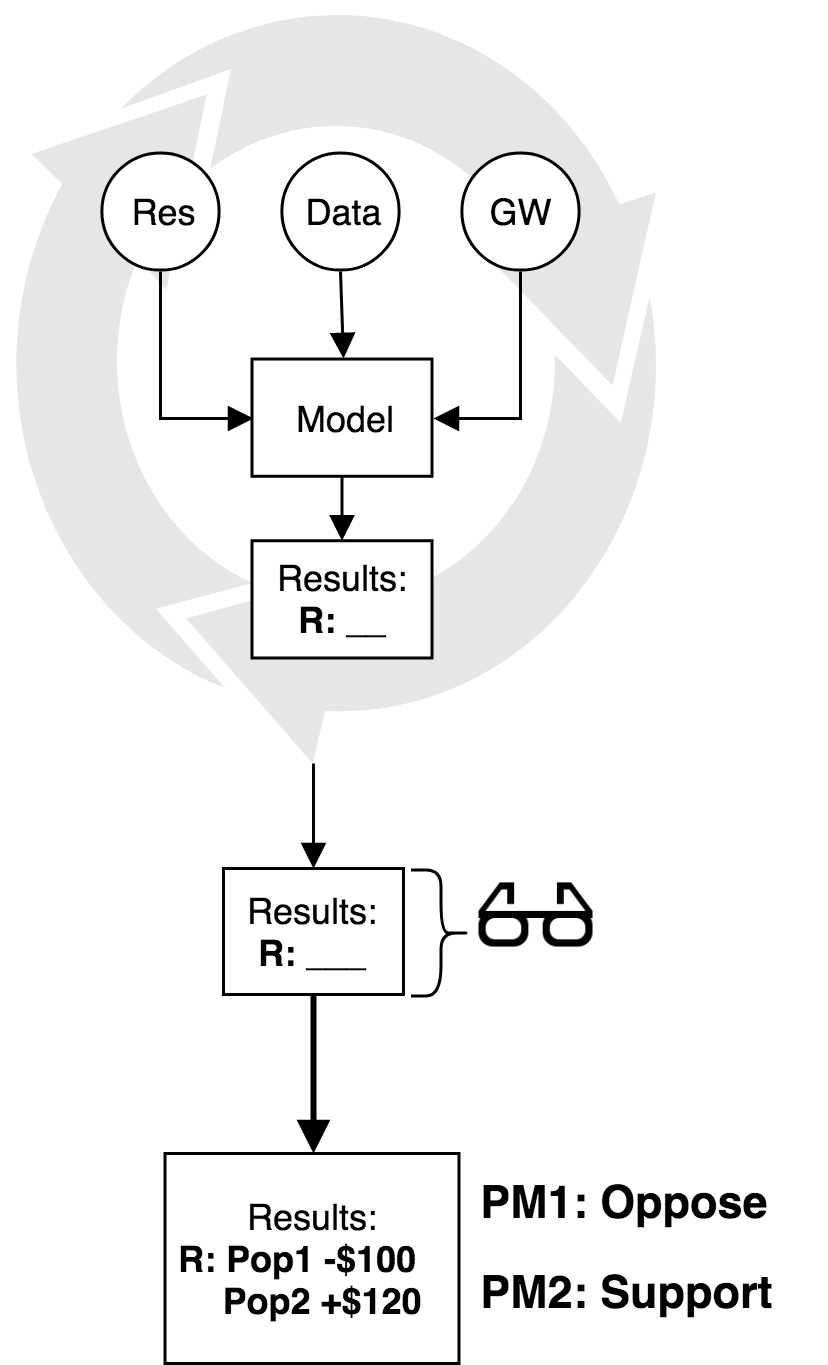
\includegraphics[width=.6\textwidth]{../Images/o_transp.png}
     \end{center}
\end{column}
\end{columns}
\end{frame}

\begin{comment}
\section{Suggestions}

\begin{frame}{Suggestions}
\textbf{Suggestions:}
\begin{enumerate}
\item \textbf{Policy Analysts: Just Post It}. \\
Things are moving in this direction. Play a leading role in a credibility revolution for policy analysis. 
\pause 
\item \textbf{Policy Analysis Organizations: Open by Default} \\
Boost in credibility, lower costs in the long run. Examples: GiveWell, and AEI. 
\pause 
\item \textbf{Government Agencies and Funders: Support Open Policy Analysis}
Examples: Require contracted policy analysis to be fully open. Support training and adoption of new tools (VC and DD). Inject resources for the transition.
\end{enumerate}
\end{frame} 
\end{comment}

\section[Conclusion]{Conclusion}

\begin{frame}{Summing Up: Where We Are}
   \begin{tikzpicture}[remember picture,overlay]
       \node[at=(current page.center), xshift = 0em, yshift = -0.5em] {
         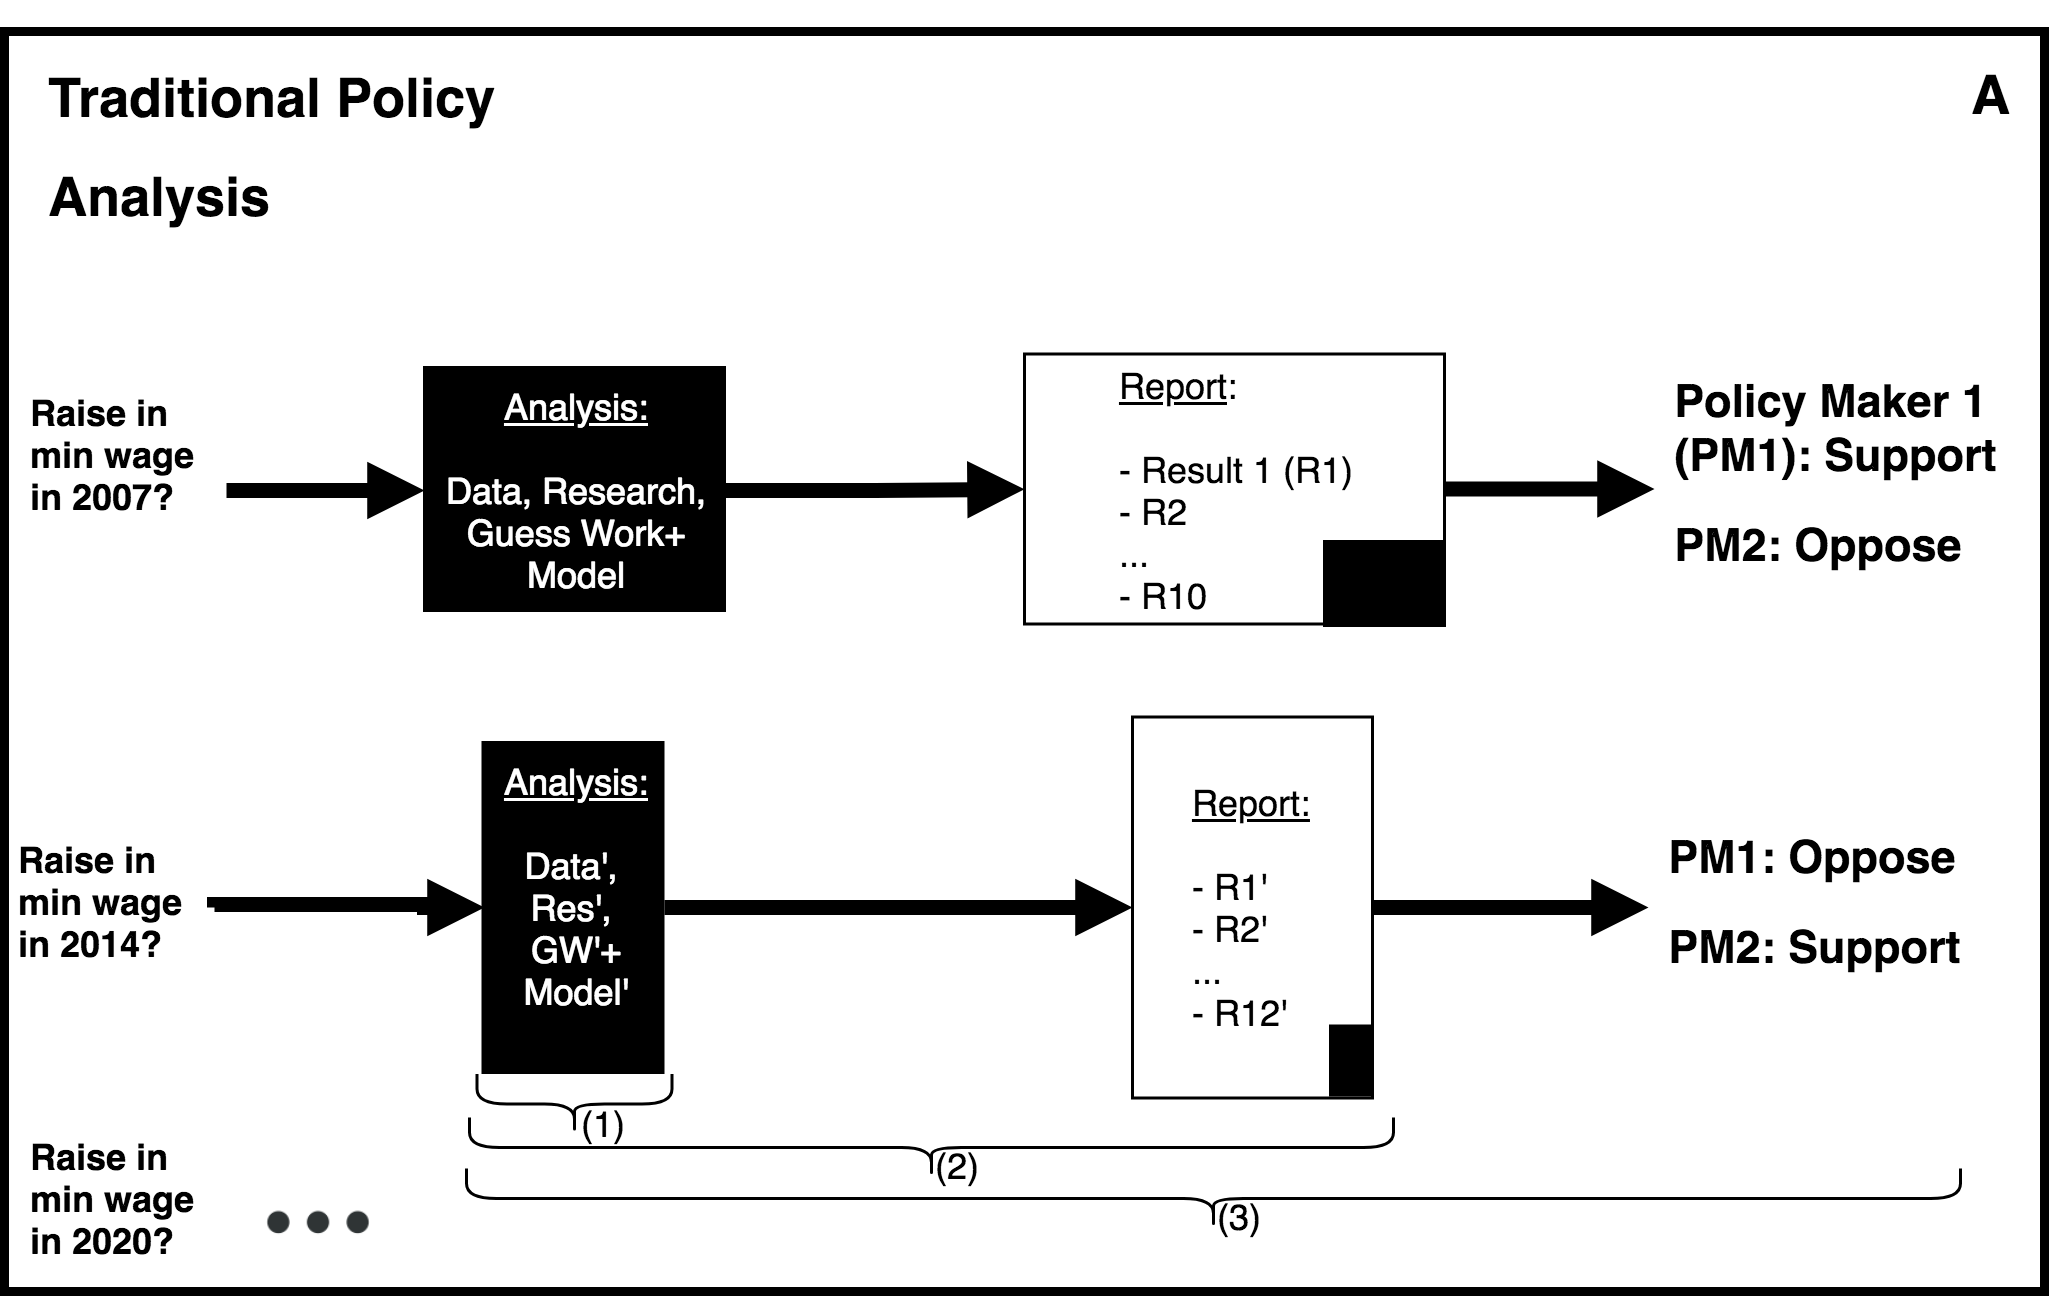
\includegraphics[width=.96\paperwidth]{../Images/traditional_pa.PNG}
       };
   \end{tikzpicture}
\end{frame}

\begin{frame}{Summing Up: Where Should We Go}
   \begin{tikzpicture}[remember picture,overlay]
       \node[at=(current page.center), xshift = 0em, yshift = -0.5em] {
         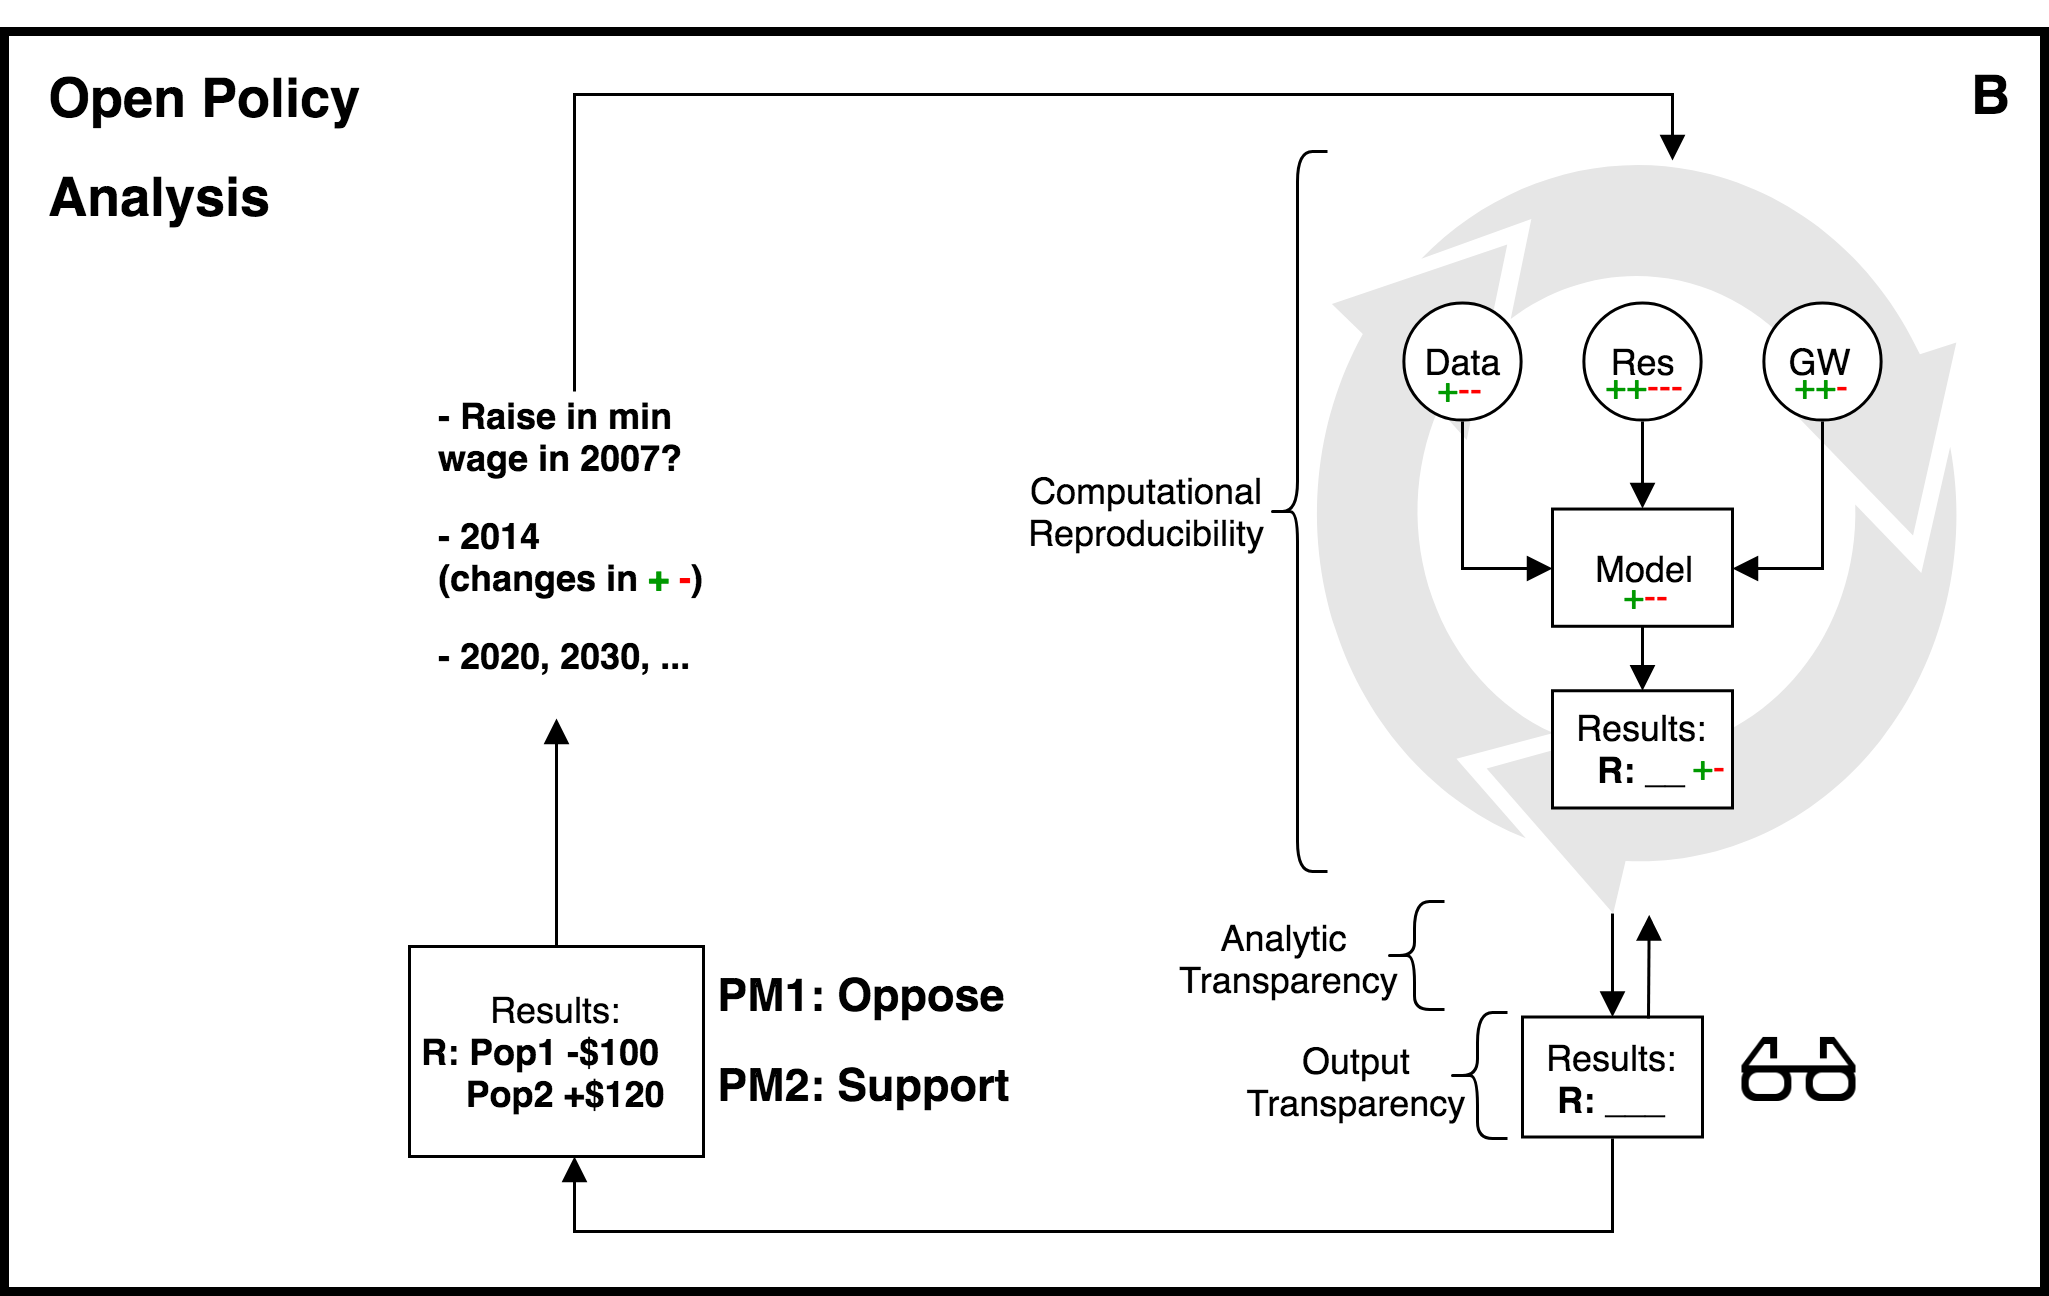
\includegraphics[width=.96\paperwidth]{../Images/open_pa.PNG}
       };
   \end{tikzpicture}
\end{frame}

%\begin{frame}{Conclusion}
%\begin{itemize}
%\item Draw a parallel between reproducibility crisis in empirical research and a credibility crisis in policy analysis. 
%\item Proposed guiding principles for open policy analysis.
%\item Identify challenges and provide recommendations for different stakeholders.
%\end{itemize}
%\end{frame}


%\begin{frame}{Next Steps} 
%\begin{itemize}
%\item Journal Science was key for research. Need high profile producer of policy analysis to buy in. 
%\item Develop community-endorsed guidelines for OPA (similar to TOP Guidelines for Open Science)
%\item Carry out case studies with policy agencies to fine tune guidelines, and build a collection of examples (Hoces de la Guardia 2017). 
%\end{itemize}
%\end{frame} 


\part{Paper 2}
\title[OPA - Minimum Wage ] % (optional, use only with long paper titles)
{Open Policy Analysis: A Case Study of the Minimum Wage Policy Estimate}

\subtitle
{}

\author[] % (optional, use only with lots of authors)
{Fernando~Hoces de la Guardia}
% - Give the names in the same order as the appear in the paper.
% - Use the \inst{?} command only if the authors have different
%   affiliation.

\institute[] % (optional, but mostly needed)
{%
  UC Berkeley:\\
  Berkeley Initiative for Transparency in the Social Sciences\\
}
% - Use the \inst command only if there are several affiliations.
% - Keep it simple, no one is interested in your street address.




\begin{frame}
  \titlepage
\end{frame}

\section{Motivation}

\begin{frame}[noframenumbering]{Motivation: Gap On How to Conduct OPA}
\begin{table}[ht]
\centering
\begin{tabular}[t]{|l|c|c|}
\hline
& Empirical  & Policy \\
& Research & Analysis \\

\hline
Problems & Reproducibility  &  Credibility \\
				 &  Crisis & Crisis \\
\hline
Solutions &  \textit{Open Science}&    \textit{Open Policy Analysis} \\
 & Principles, Guidelines,  &   Principles{\white, \textbf{Guidelines,}}\\
 & Applications &   {\white \textbf{Applications}}\\

\hline
\end{tabular}
\end{table}%
\end{frame}


\begin{frame}[noframenumbering]{Motivation: Gap On How to Conduct OPA}
\begin{table}[ht]
\centering
\begin{tabular}[t]{|l|c|c|}
\hline
& Empirical  & Policy \\
& Research & Analysis \\

\hline
Problems & Reproducibility  &  Credibility \\
				 &  Crisis & Crisis \\
\hline
Solutions &  \textit{Open Science}&    \textit{Open Policy Analysis} \\
 & Principles, Guidelines,  &   Principles, Guidelines,\\
 & Applications &   Applications\\

\hline
\end{tabular}
\end{table}%
\end{frame}
 
% \section{Approach}
%\begin{frame}{Approach}
%\begin{itemize}
%item Identify a case study
%\item Define guidelines
%\item Demonstrate how to achieve highest standards of Open Policy Analysis (OPA)
%\item Use sensitivity analysis to explore biggest policy unknowns 
%\begin{itemize}
%\item  Surprisingly, academic debate around one specific parameter seems less relevant from policy perspective
%\end{itemize}
%\end{itemize}
%\end{frame} 

\section[Case Study]{Description of Case Study}

\begin{frame}[label =  desc_cs]{Description of Case Study}
% 4mins
\begin{center}
``The Effects of a Minimum-Wage Increase on Employment and Family Income'' 
Congressional Budget Office (2014)
\end{center}

\textbf{Description:} CBO estimated the effects of a raise in the federal minimum wage from \$7.25/hr to \$10.10/hr. 


\textbf{Main policy estimates:}
\begin{itemize}
\item ~500,000 jobs would be lost.
\item 16.5 million workers would receive a salary increase. 
\item Distributional effects: below poverty line (PL) +\$5billion; between one and three PL +\$12billion; between three and six PL +\$2billion; above six PL -\$17billion
\end{itemize}

\textbf{Key research estimate:} Elasticity of labor demand for teenagers in the labor force. 
\end{frame}

\begin{comment}

\begin{frame}{Reasons for Selecting the Case Study}
    \begin{multicols}{2}
    \begin{itemize}
        \item Scalable
        \item Recurrent
        \item Feasible
        \item Relevant:
    \end{itemize}
    \end{multicols}
\begin{figure}[h!]
\centering
\vspace*{-1em}
\hspace*{-1.7em}
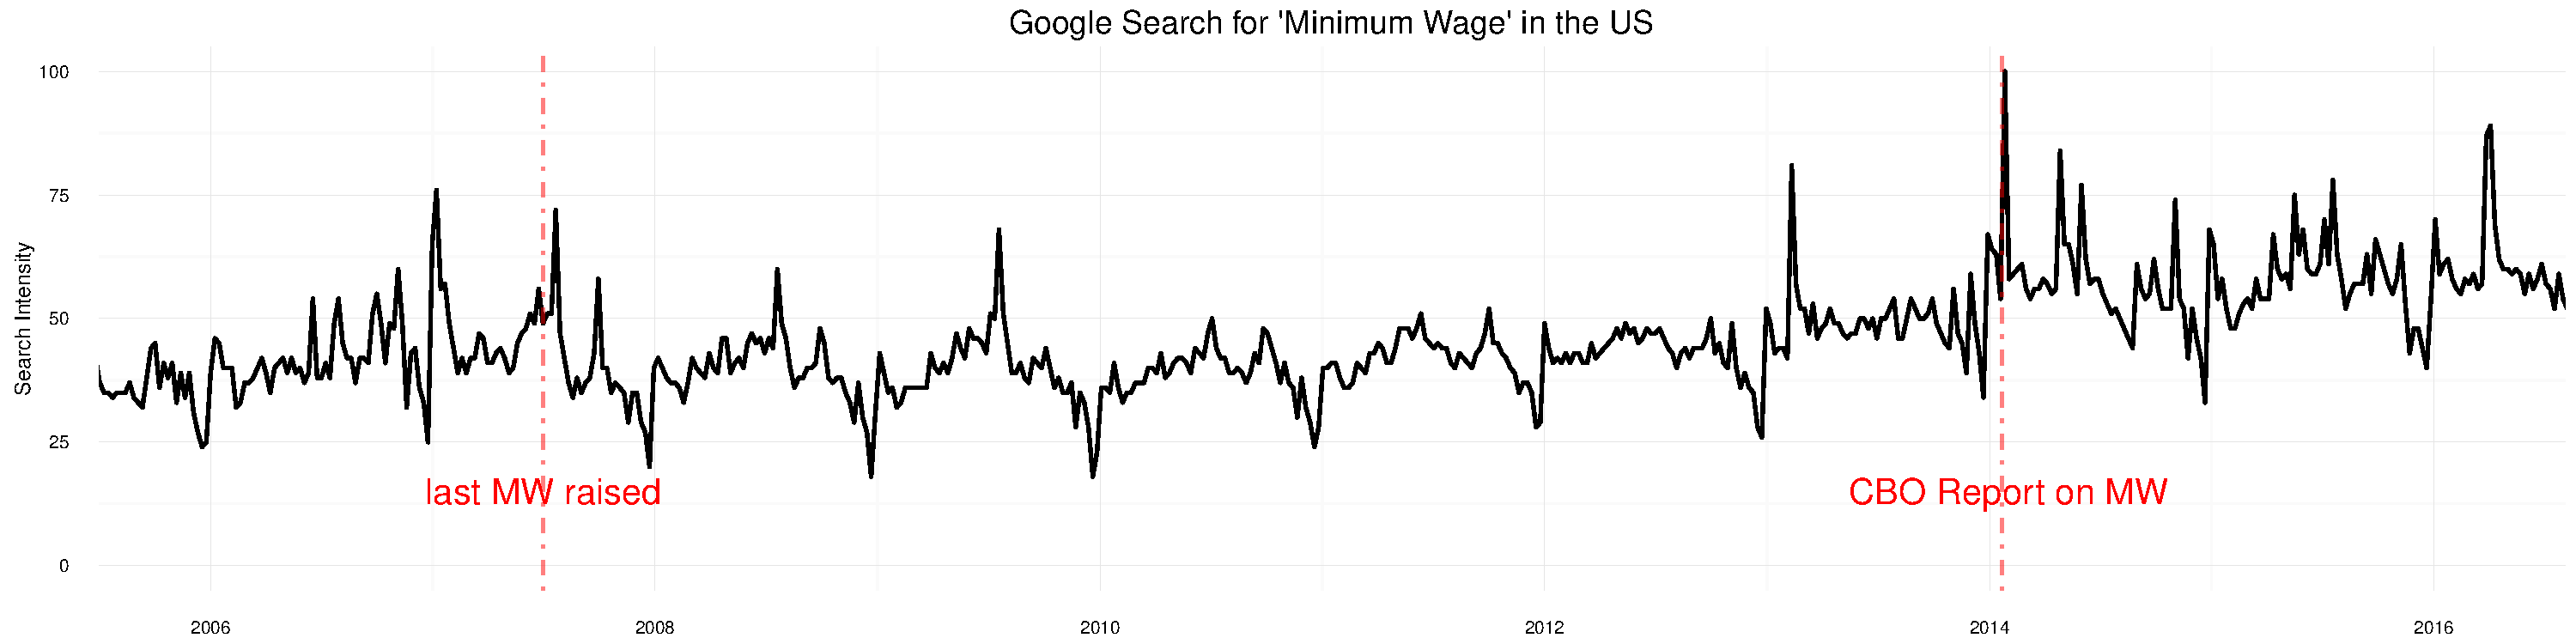
\includegraphics[scale = 0.22]{../Images/min_wage_gtrend}
\vspace*{-0.8em}
\caption{Google Search Intensity of ``Minimum Wage''}
\label{mw_gtrend}
\end{figure}	
\end{frame}

\end{comment}

\section{Guidelines}



\begin{frame}{Summary of Adapted Guidelines}
 \centering
 \resizebox{25em}{10em}{%
    \begin{tabular}{ P{1.2cm} P{2cm} P{3cm}  P{3cm}  P{3cm} }
     \toprule
     {\black Standard} & {\black Level 0} 	& {\black Level 1} & {\black Level 2} & {\black Level 3} \\
     \midrule      \midrule
   {\black Workflow} & {\gray Policy estimates vaguely described}  & {\gray All the inputs, and their corresponding sources, used in the calculations are listed } & {\gray Lvl 1 + Policy estimates are listed, in same unit if possible} & {\gray Lvl 2 + all the components can be modified with little effort} \\
     \midrule
    {\black Data} & {\gray Report says nothing} & {\gray Clearly stated whether all, some components, or none of the data is available, with instructions for access when possible.} & {\gray Lvl 1 + report and data are in same place} & {\gray Lvl 2 + Report has specific lines of code that call the data and changes in the data produce traceable changes in the report} \\
     \midrule
      {\black Methods \& Code} & {\gray Key assumption are listed} & {\gray Methods are described in prose. Large amount of work is required to reproduce qualitatively similar estimates}  & {\gray Methods and described in prose, with detailed formulas, and code is provided as supplementary material} & {\gray Lvl 2 + All is in the same document where changes in the code affect the output automatically} \\
     \toprule
     \multicolumn{5}{ P{11.7cm} }{  \raggedleft {\black\small{ From TOP guidelines (Nosek et al 2015) v1.0.1}} \small{\hyperlink{no_gray}{\beamerbutton{}}} }
   \end{tabular}}
\end{frame}


\begin{frame}[noframenumbering]{Summary of Adapted Guidelines}
 \centering
 \resizebox{25em}{10em}{%
    \begin{tabular}{ P{1.2cm} P{2cm} P{3cm}  P{3cm}  P{3cm} }
     \toprule
    {\black Standard} & {\red Level 0 } 	&  {\red Level 1 } &  {\red Level 2}  & {\red Level 3 }  \\
     \midrule      \midrule
    {\black Workflow} & {\gray Policy estimates vaguely described}  & {\gray All the inputs, and their corresponding sources, used in the calculations are listed } & {\gray Lvl 1 + Policy estimates are listed, in same unit if possible} & {\gray Lvl 2 + all the components can be modified with little effort} \\
     \midrule
    {\black Data} & {\gray Report says nothing} & {\gray Clearly stated whether all, some components, or none of the data is available, with instructions for access when possible.} & {\gray Lvl 1 + report and data are in same place} & {\gray Lvl 2 + Report has specific lines of code that call the data and changes in the data produce traceable changes in the report} \\
     \midrule
      {\black Methods \& Code} & {\gray Key assumption are listed} & {\gray Methods are described in prose. Large amount of work is required to reproduce qualitatively similar estimates}  & {\gray Methods and described in prose, with detailed formulas, and code is provided as supplementary material} & {\gray Lvl 2 + All is in the same document where changes in the code affect the output automatically} \\
     \toprule
     \multicolumn{5}{ P{11.7cm} }{  \raggedleft {\black\small{ From TOP guidelines (Nosek et al 2015) v1.0.1}} \small{\hyperlink{no_gray}{\beamerbutton{}}} }
   \end{tabular}}
\end{frame}


\begin{frame}[noframenumbering]{Summary of Adapted Guidelines}
 \centering
 \resizebox{25em}{10em}{%
    \begin{tabular}{ P{1.2cm} P{2cm} P{3cm}  P{3cm}  P{3cm} }
     \toprule
     {\red Standard} & {\black Level 0} 	& {\black Level 1} & {\black Level 2} & {\black Level 3} \\
     \midrule      \midrule
    {\red Workflow} & {\gray Policy estimates vaguely described}  & {\gray All the inputs, and their corresponding sources, used in the calculations are listed} & {\gray Lvl 1 + Policy estimates are listed, in same unit if possible} & {\gray Lvl 2 + all the components can be modified with little effort} \\
     \midrule
    {\red Data} & {\gray Report says nothing} & {\gray Clearly stated whether all, some components, or none of the data is available, with instructions for access when possible.} & {\gray Lvl 1 + report and data are in same place} & {\gray Lvl 2 + Report has specific lines of code that call the data and changes in the data produce traceable changes in the report} \\
     \midrule
      {\red Methods \& Code} & {\gray Key assumption are listed} & {\gray Methods are described in prose. Large amount of work is required to reproduce qualitatively similar estimates}  & {\gray Methods and described in prose, with detailed formulas, and code is provided as supplementary material} & {\gray Lvl 2 + All is in the same document where changes in the code affect the output automatically} \\
     \toprule
     \multicolumn{5}{ P{11.7cm} }{  \raggedleft {\black\small{ From TOP guidelines (Nosek et al 2015) v1.0.1}} \small{\hyperlink{no_gray}{\beamerbutton{}}} }
   \end{tabular}}
\end{frame}

\begin{frame}[noframenumbering, label=guidelines_sum]{Summary of Adapted Guidelines}
 \centering
 \resizebox{25em}{10em}{%
    \begin{tabular}{ P{1.2cm} P{2cm} P{3cm}  P{3cm}  P{3cm} }
     \toprule
     Standard & Level 0 	& Level 1 & Level 2 & Level 3 \\
     \midrule      \midrule
   {\black Workflow} & {\gray Policy estimates vaguely described}  & {\gray All the inputs, and their corresponding sources, used in the calculations are listed } & {\gray Lvl 1 + Policy estimates are listed, in same unit if possible} & {\gray Lvl 2 + all the components can be modified with little effort} \\
     \midrule
    {\black Data} & {\gray Report says nothing} & {\gray Clearly stated whether all, some components, or none of the data is available, with instructions for access when possible.} & {\gray Lvl 1 + report and data are in same place} & {\gray Lvl 2 + Report has specific lines of code that call the data and changes in the data produce traceable changes in the report} \\
     \midrule
      {\black Methods \& Code} & {\gray Key assumption are listed} & {\gray Methods are described in prose. Large amount of work is required to reproduce qualitatively similar estimates}  & {\gray Methods and described in prose, with detailed formulas, and code is provided as supplementary material} & {\gray Lvl 2 + All is in the same document where changes in the code affect the output automatically} \\
     \toprule
     \multicolumn{5}{ P{11.7cm} }{  \raggedleft {\red\small{ From TOP guidelines (Nosek et al 2015) v1.0.1}} \small{\hyperlink{no_gray}{\beamerbutton{}}} }
   \end{tabular}}
\end{frame}

\section{Application}




\begin{frame}[label=demo]{Applying Guidelines to Build an Open Report}
\begin{center}

{\Huge
\texttt{\href{https://rpubs.com/fhoces/dd_cbo_mw}{{\blue\underline{DEMO}}}}
}\small{\hyperlink{no_inet}{\beamerbutton{}}}


\end{center}

%Discuss automation 

\end{frame}

\begin{comment}

\begin{frame}[shrink=25, label=map_cbo]{Map the complete policy analysis}

\tikzstyle{estimate} = [diamond, draw, node distance= 7em,text width = 5em, minimum height=5em, minimum width=5em, align = center]
\tikzstyle{line} = [draw, -stealth]
\tikzstyle{line_enph} = [draw, red, ultra thick]
\tikzstyle{inp} = [draw, rectangle, text centered, minimum height=3em, text width=2em, node distance= 2em]
\tikzstyle{source} = [draw, rectangle, text centered, minimum height=8em, text width=5em, node distance= 10em]
\tikzstyle{model} = [draw, rectangle, text centered, minimum height=8em, text width=15em, node distance= 10em]
%\tikzstyle{outp} = [draw, ellipse, text centered, minimum height=2mm, text width=2em, node distance= 10em]
%\tikzstyle{block} = [draw, rectangle,  text width=8em, text centered, minimum height=55mm, node distance= 5em]


\begin{figure}[h!]\centering \label{pa_components_ex}
\hspace*{-2.5em}
\begin{tikzpicture}[thick,scale=0.6, every node/.style={scale=0.6}]
\setbeamercovered{invisible}

%%%%%Nodes: Sources%%%%%%%
\node [source](D_1){CPS ORG; CPS ASEC; CBO 10-Y projections};
\node [source, below = 1em of D_1](Lit){Labor demand for teenagers; Ripple effects};
\node [source, below = 1em of Lit](OR){Extrap. for adults; Aggregate effects; Dist of losses};


\draw[decoration={brace,mirror}, decorate] (-1.2,-10) -- node[below=6pt] {$Sources$}(1.1,-10);

\draw[decoration={brace,mirror}, decorate] (4.8,-11.3) -- node[below=6pt] {$Inputs$}(6.2,-11.3);


%node[below = 1em ](OR) -- node[below = 6em]{asd}(OR)



%%%%%Nodes: Inputs%%%%%%%
\node [inp, above right = 1em and 6em of  D_1 ](I_1){$dF_{w}$};
\node [inp, below = 1em of I_1](I_2){$g_{N}$};
\node [inp, below = 10em of I_2](I_j){$\eta_{teens}$};
\node [inp, below right = 1em and 6em of OR ](I_last){$F_{ext}$};



\path (I_2) -- node[auto=false, rotate=90, anchor=north, outer sep=-0.5em]{\ldots} (I_j);
\path (I_j) -- node[auto=false, rotate=90, anchor=north, outer sep=-0.5em]{\ldots} (I_last);

%%%%%Paths connecting Sources with Inputs%%%%%%%
\draw [line](D_1.east) -- (I_1.west);
\draw [line](D_1.east) -- (I_2.west);
\draw [line, opacity=1, anchor=center](Lit.east) -- (I_j.west);
\draw [line, opacity=1, anchor=center](OR.east) -- (I_last.west);

\draw [line, opacity=.3][xshift=1em](D_1.east) -- ([yshift=-8 em]I_1.west);
\draw [line, opacity=.3][xshift=1em](D_1.east) -- ([yshift=-10 em]I_1.west);

\draw [line, opacity=.3][xshift=1em](Lit.east) -- ([yshift=7 em]I_j.west);
\draw [line, opacity=.3][xshift=1em](Lit.east) -- ([yshift=-3 em]I_j.west);

\draw [line, opacity=.3][xshift=1em](OR.east) -- ([yshift=3 em]I_last.west);
\draw [line, opacity=.3][xshift=1em](OR.east) -- ([yshift=5 em]I_last.west);


%%%%%Node and paths for model%%%%%%%
\node [model, below right = 2em and 10em of D_1](model){\hyperlink{equations}{Equations}: \ref{N_final} - \ref{last.eq} };
\draw [line](I_1) -| (model);
\draw [line](I_2) -| (model);
\draw [line](I_j) |- (model);
\draw [line](I_last) -| (model);

%%%%%Node and paths for policy estimates%%%%%%%
\node [estimate, right = 5em of model](PE_2){Average wage gain};
\node [estimate, above = 5em of PE_2](PE_1){Average wage loss};
\node [estimate, below = 5em of PE_2](PE_3){Average balance loss};


\draw [line] (model.east) -- (PE_1.south west);
\draw [line] (model.east) -- (PE_2.west);
\draw [line] (model.east) -- (PE_3.north west);


\end{tikzpicture}
\end{figure}
\hyperlink{full_model}{\beamerbutton{}}
\hyperlink{equations}{\beamerbutton{}}
\hyperlink{before}{\beamerbutton{}}
\end{frame}

\begin{frame}{All in One Output 1/3}
\begin{figure}[h!]
\centering
\hspace*{-3em}
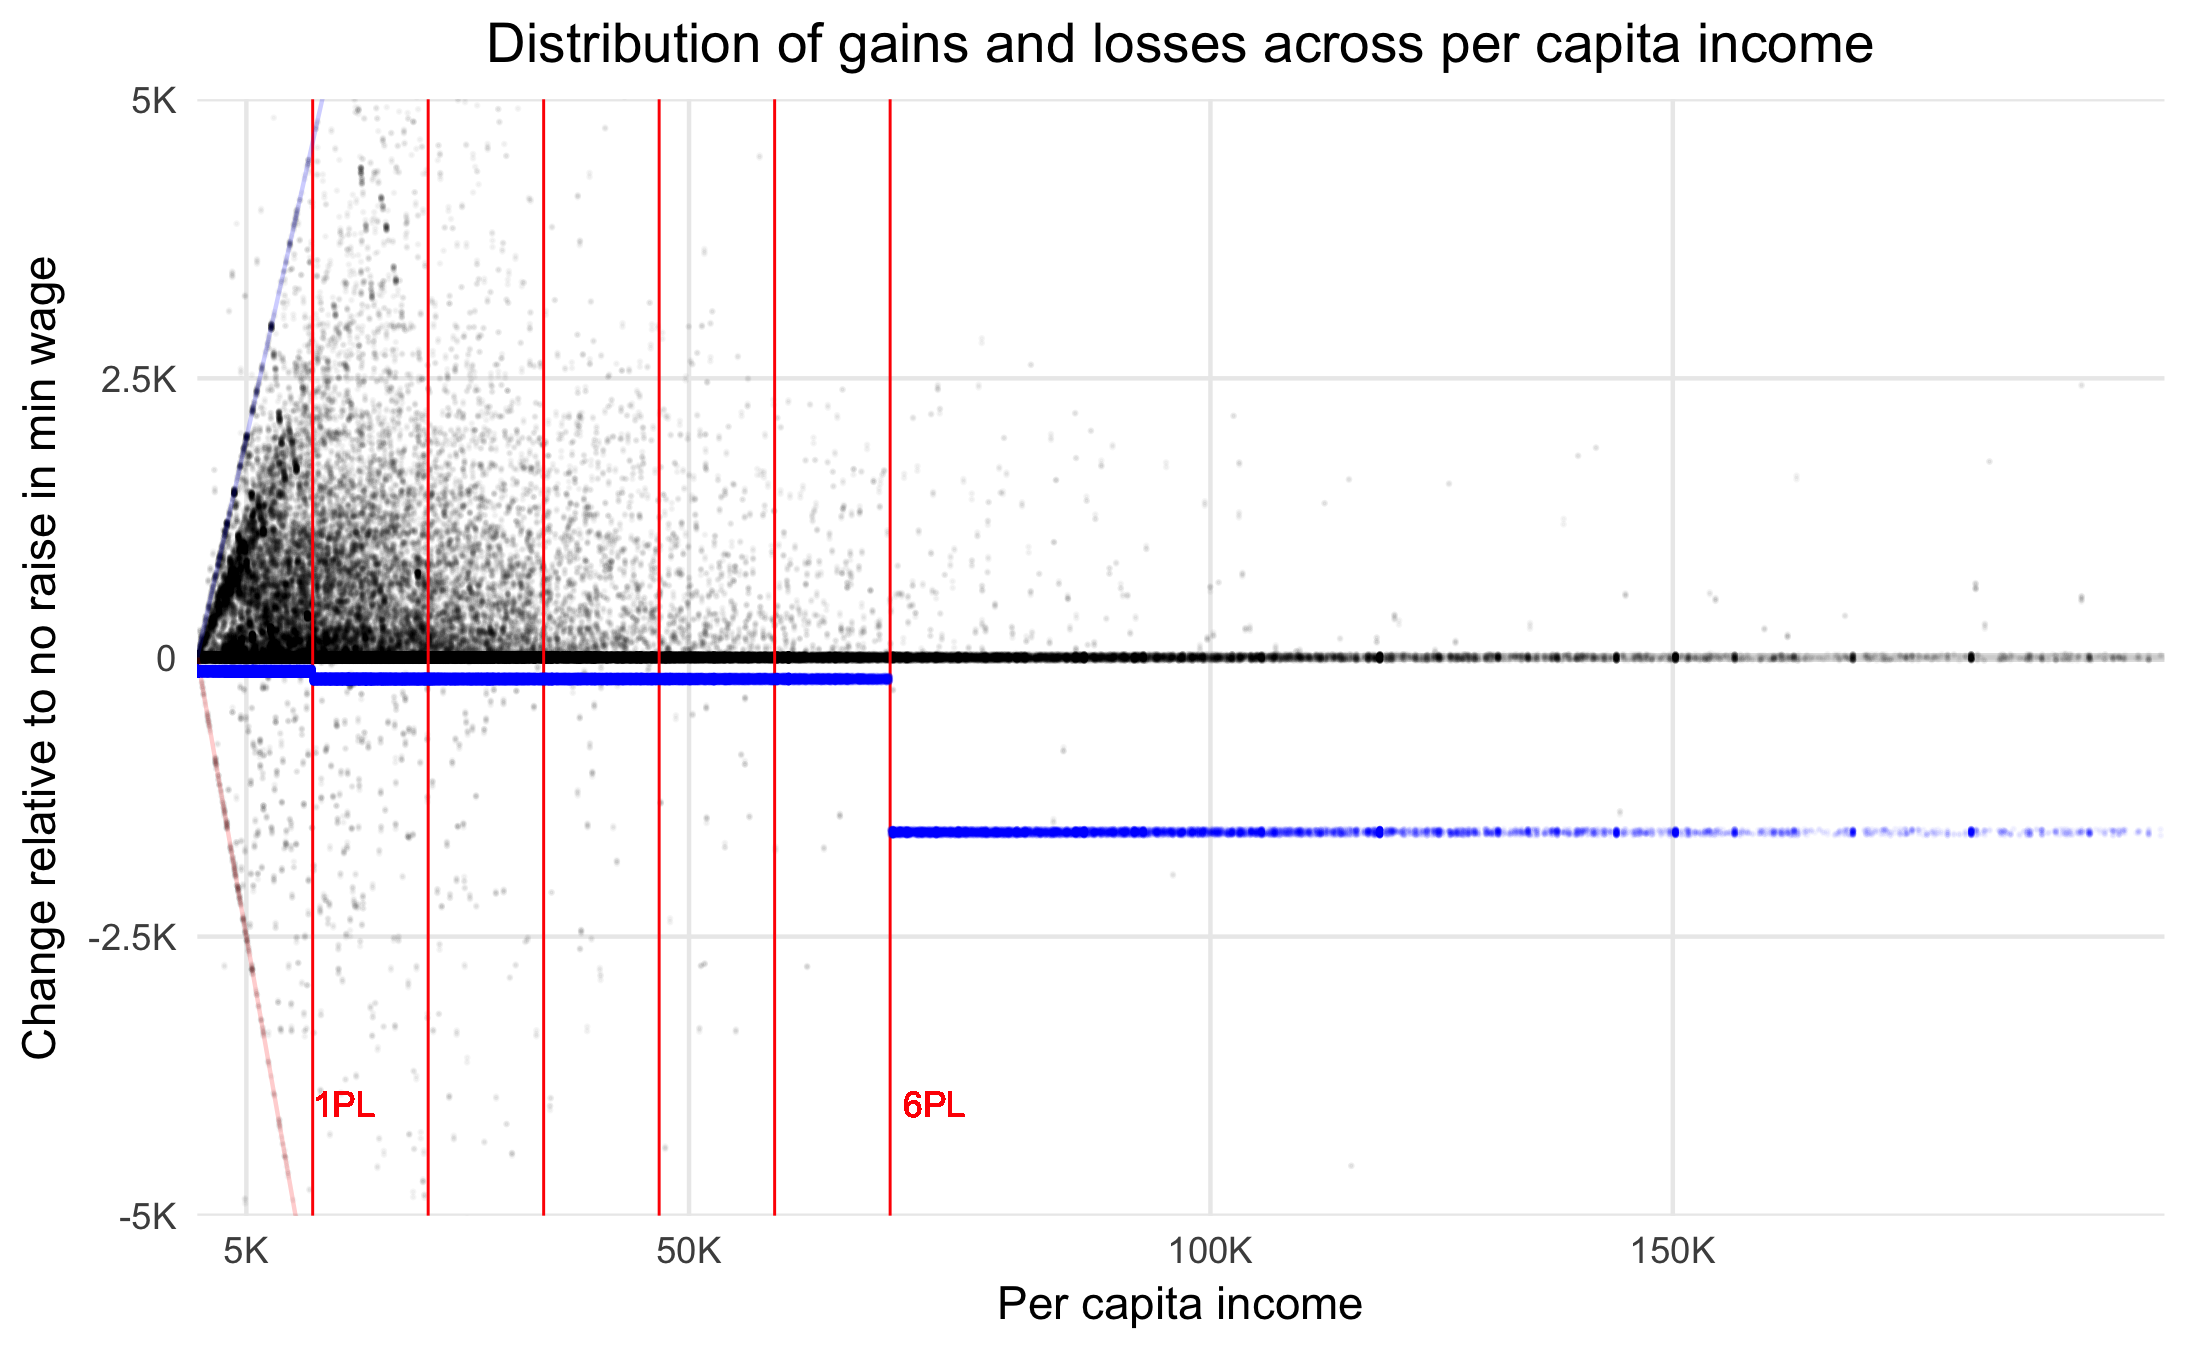
\includegraphics[scale = 0.13]{../Images/alt_pe1}
\caption{Gains and losses. Different Units}
\end{figure}	
\end{frame}

\begin{frame}{All in One Output 2/3}
\begin{figure}[h!]
\centering
\hspace*{-3em}
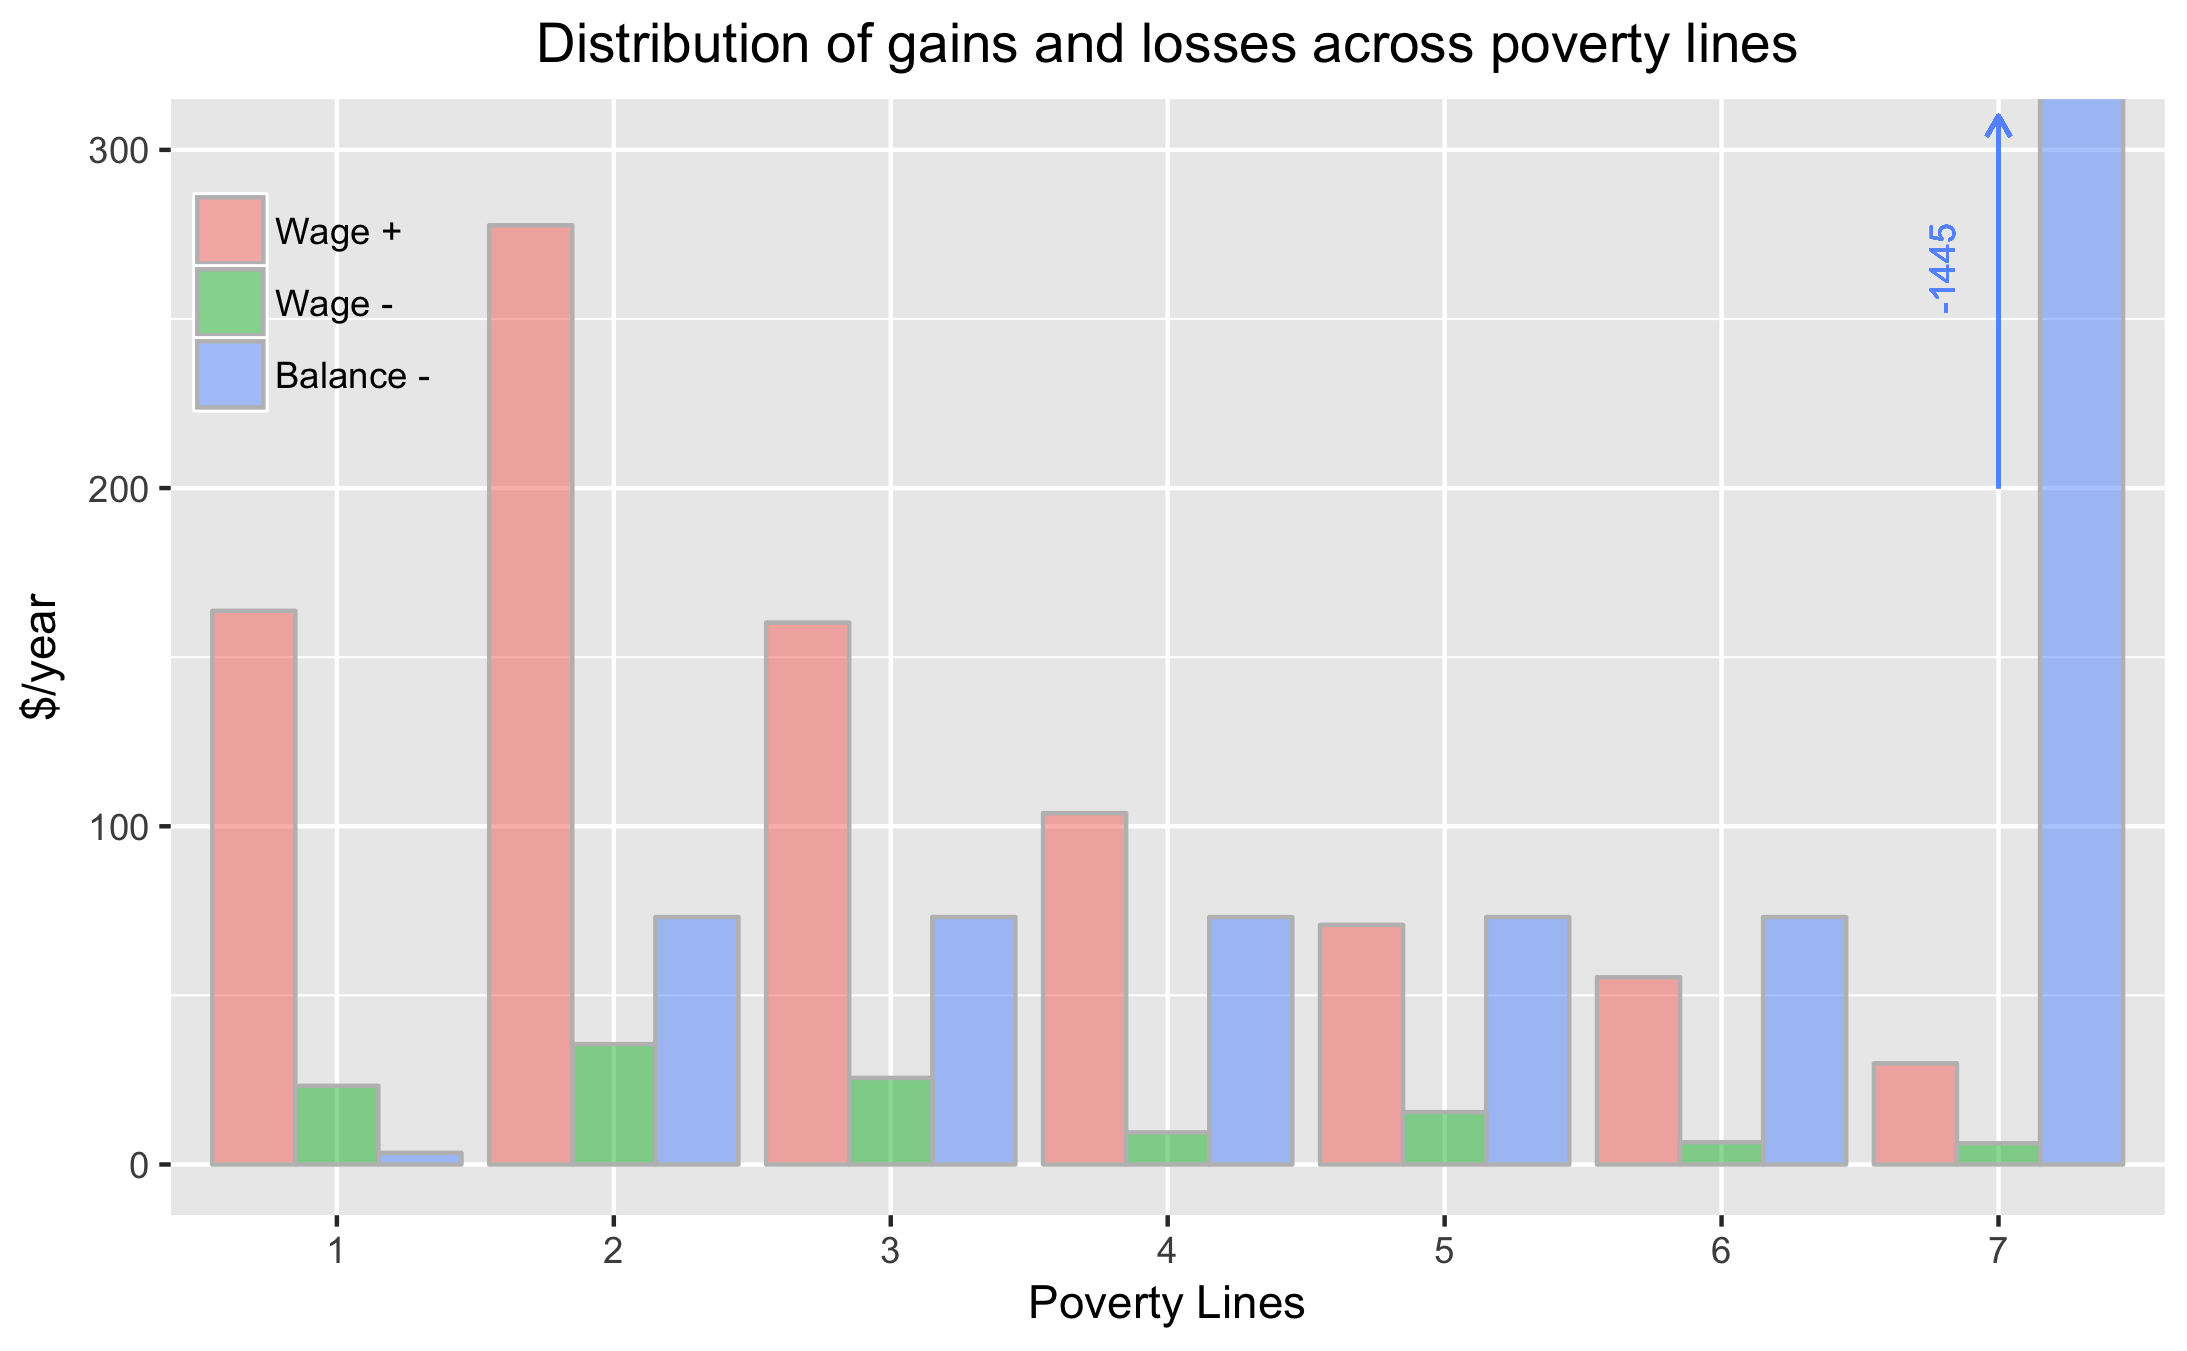
\includegraphics[scale = 0.13]{../Images/alt_pe2}
\caption{Gains and losses. Different Denominator}
\end{figure}	
\end{frame}

\begin{frame}{All in One Output 3/3}
\begin{figure}[h!]
\centering
\hspace*{-3em}
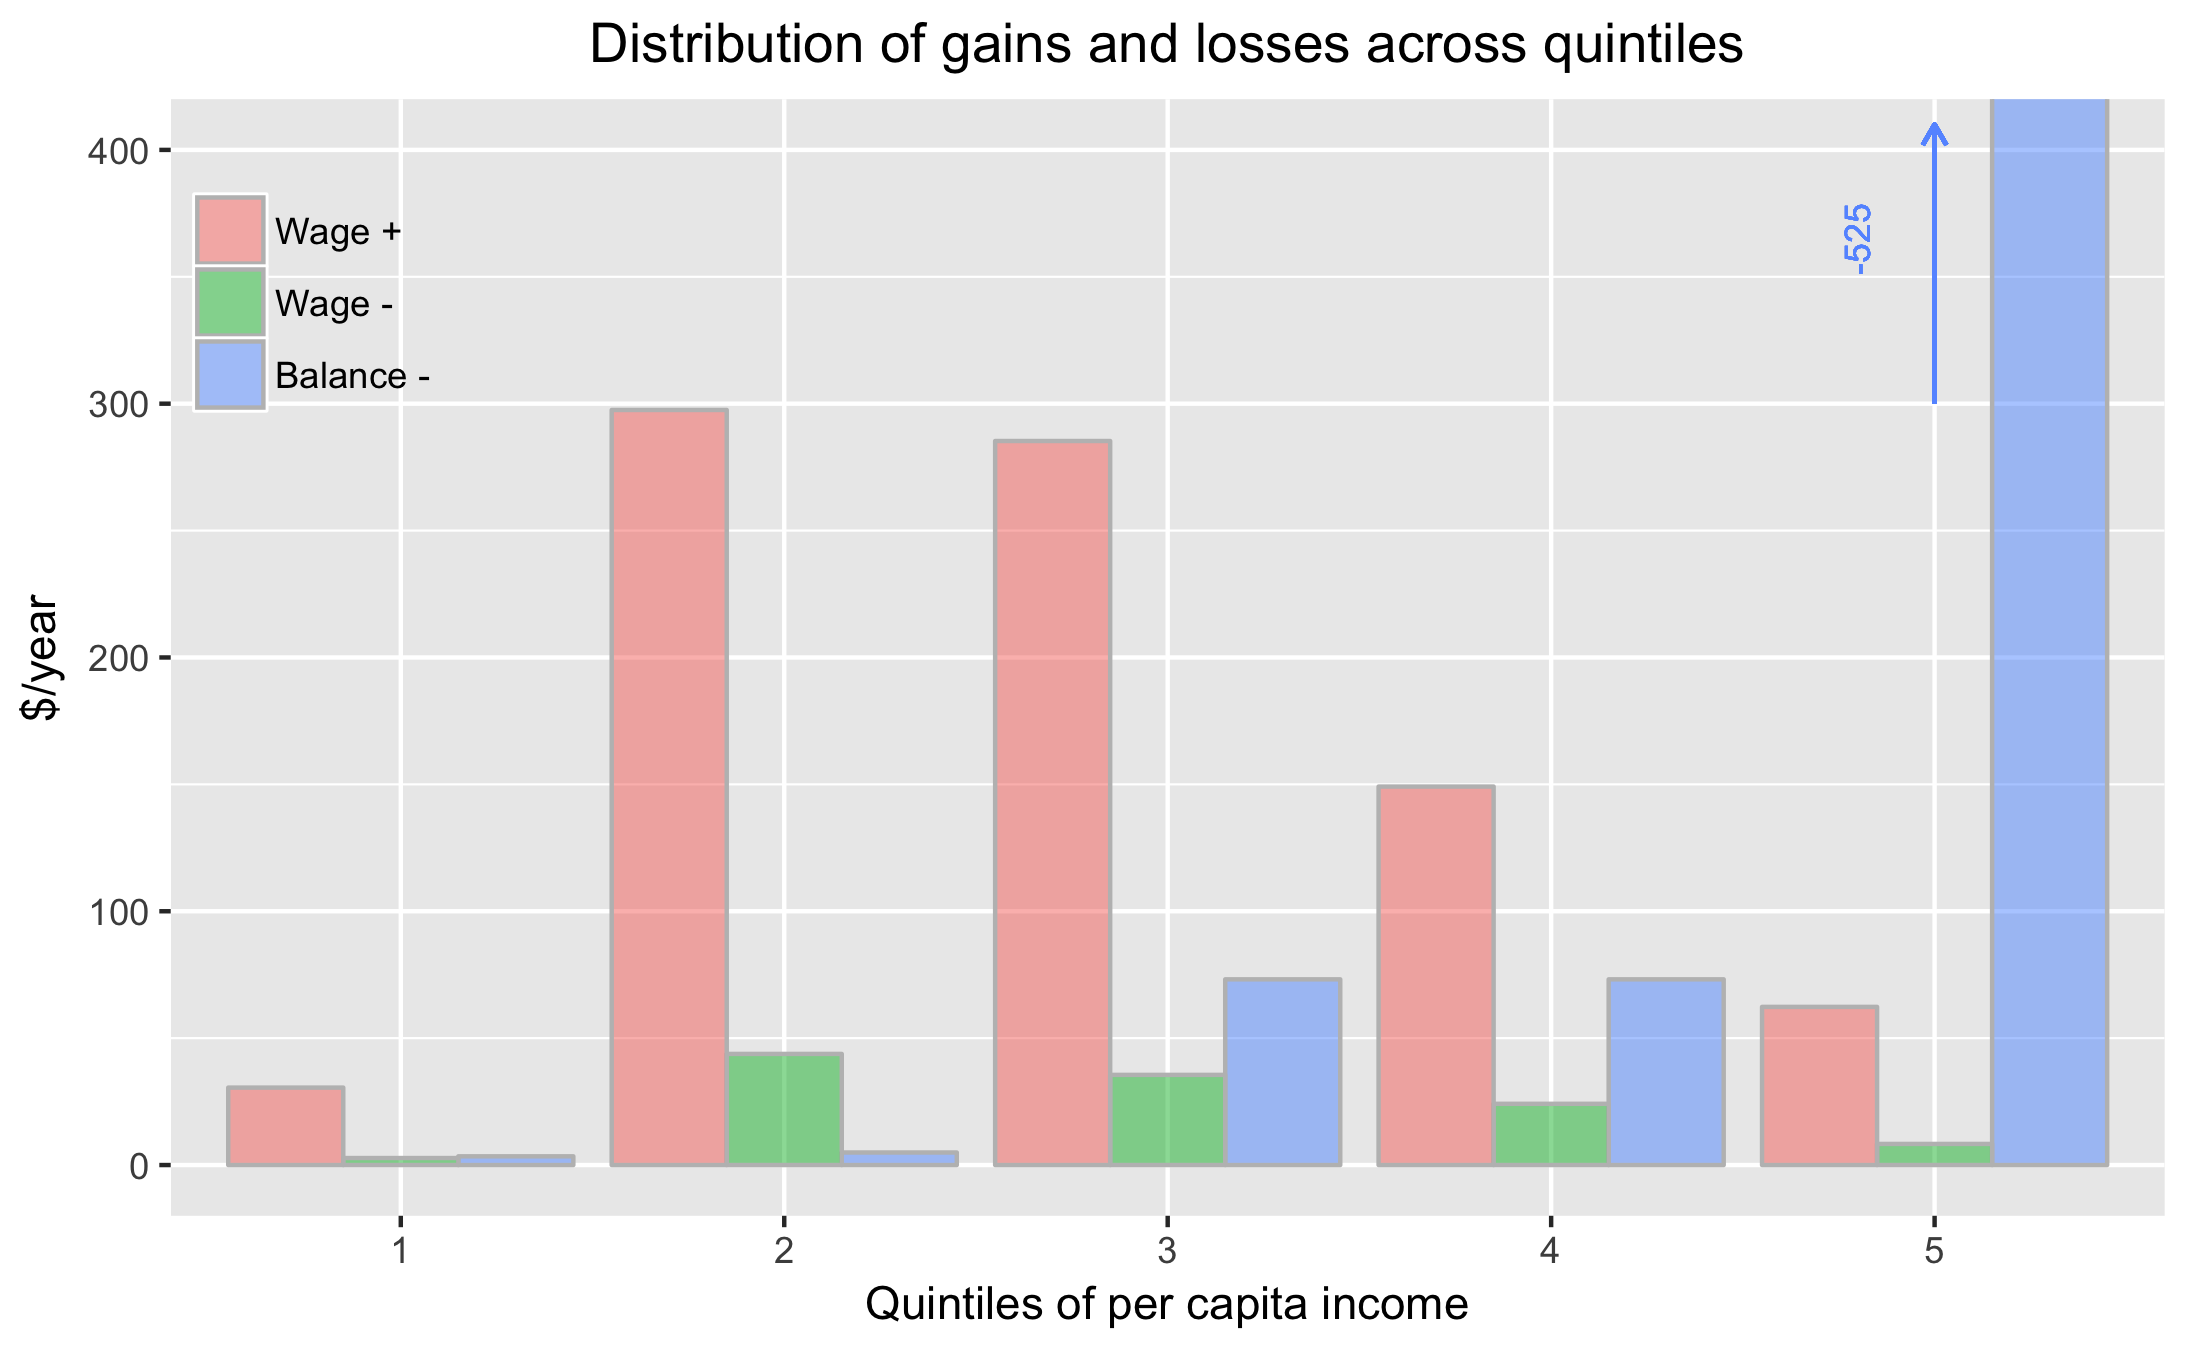
\includegraphics[scale = 0.13]{../Images/policy_est}
\caption{Gains and losses. Same units and denominator}
\end{figure}	
\end{frame}

\end{comment}


\begin{frame}{Demo Checklist}
\begin{itemize}
\item One-click reproducible \& machine independent.
\item WYSIATI.
\item Readable. Weather you know {\large\texttt{R}} or not. 
\item TO DO: diff between two versions.
\item Sensitivity analysis.
\end{itemize}
\end{frame}

\section{Sensitivity Analysis}

\begin{frame}[noframenumbering]{Sensitivity Analysis: Status Quo}
\begin{figure}[h!]
\centering
\hspace*{-3em}
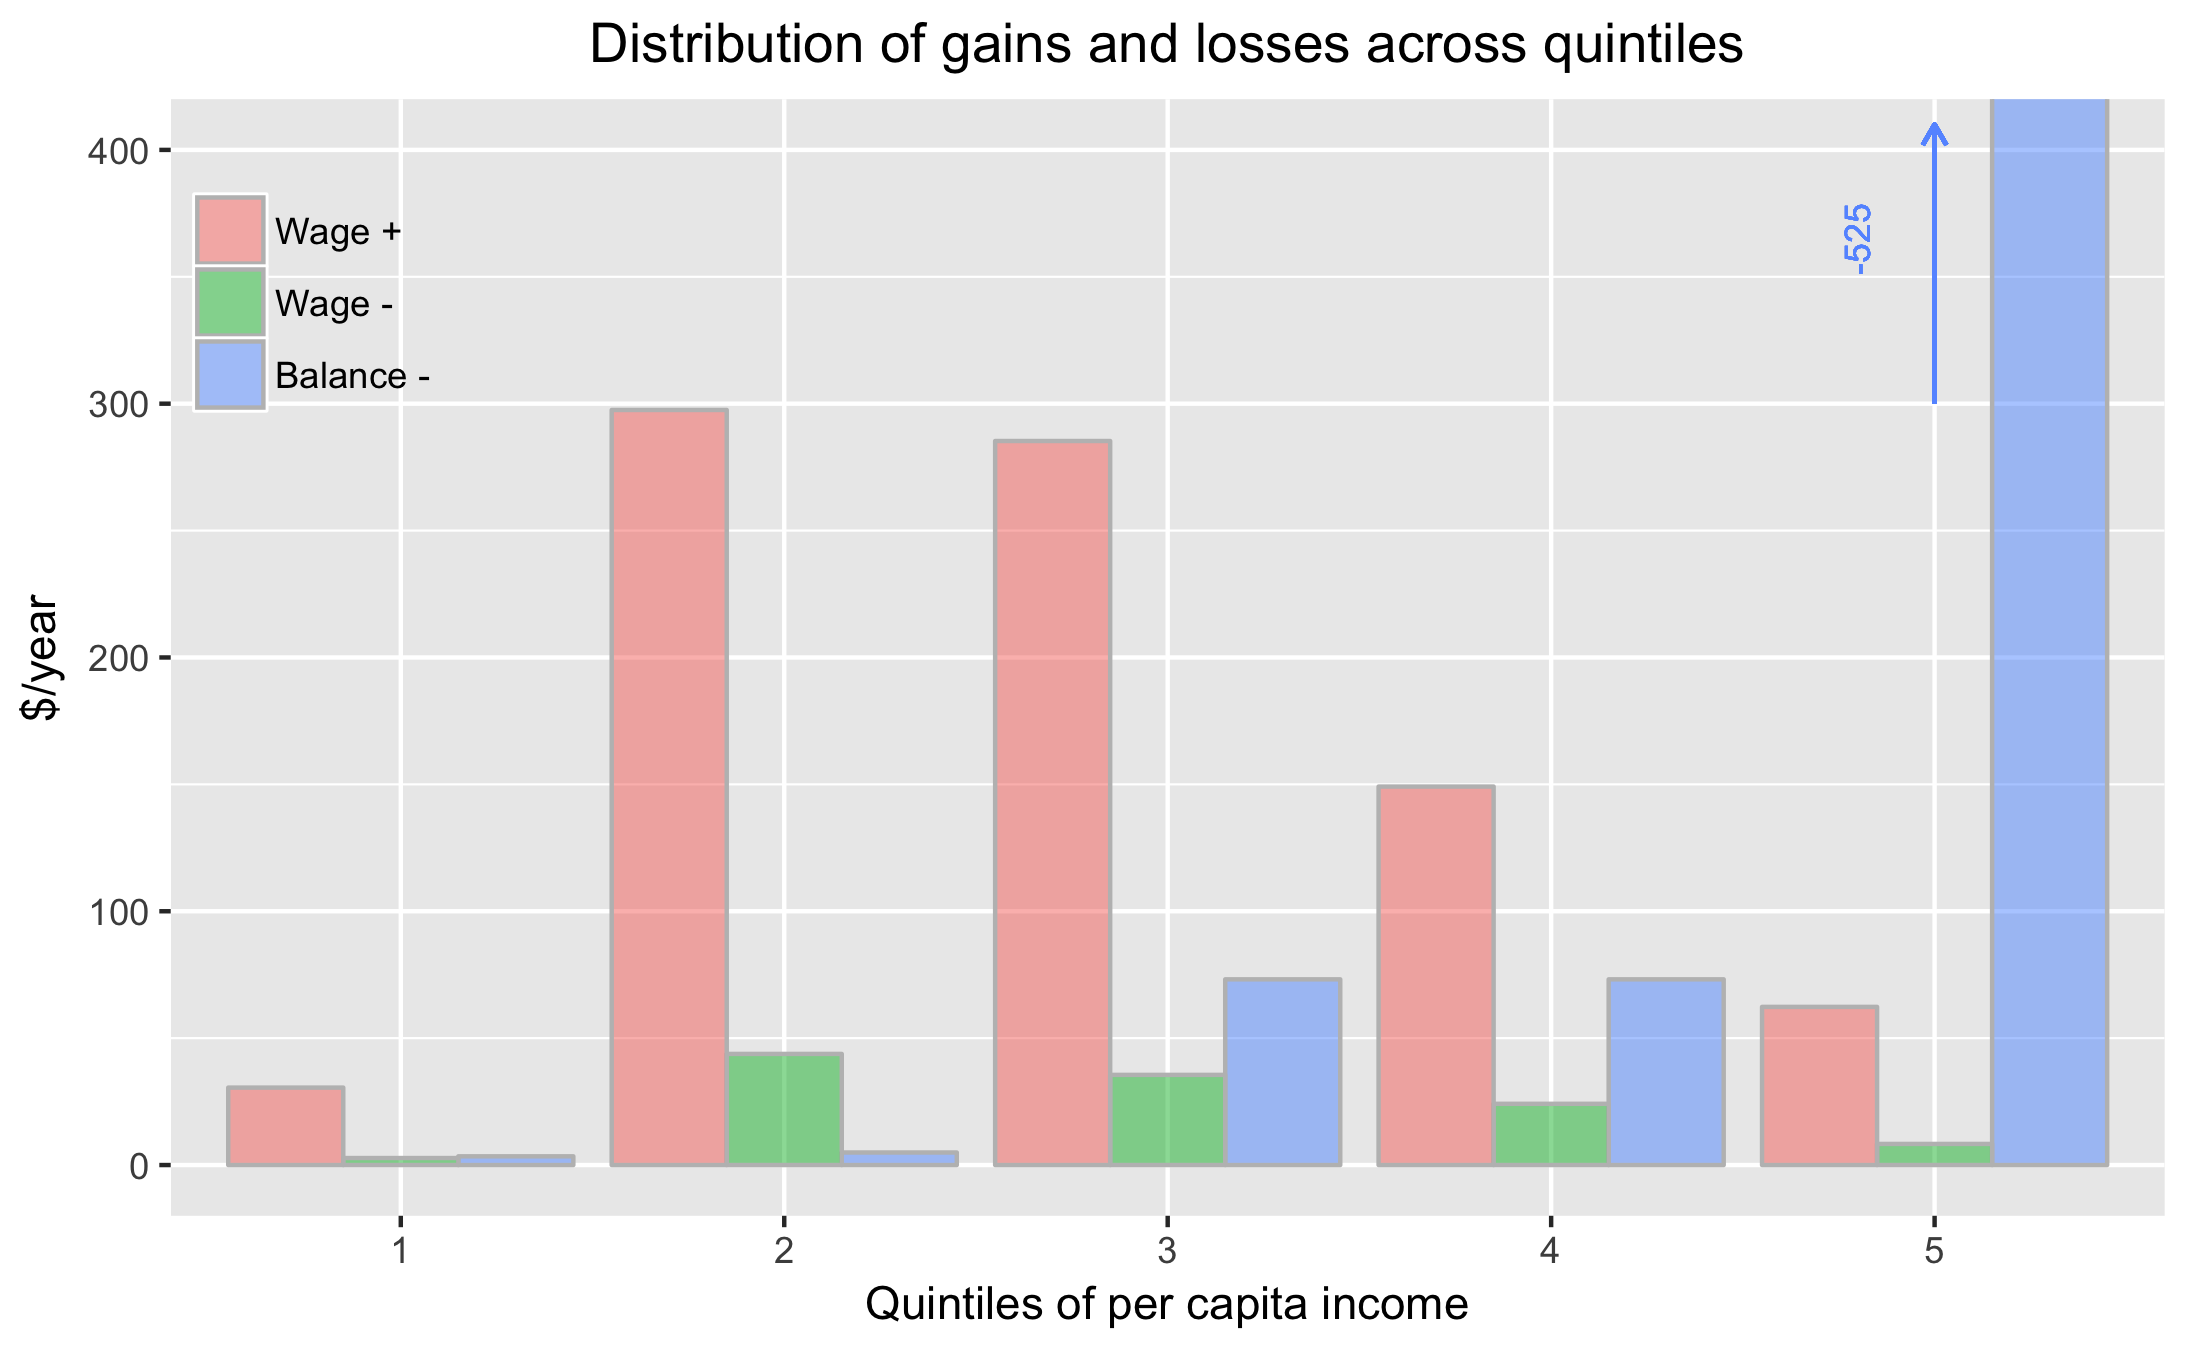
\includegraphics[scale = 0.13]{../Images/policy_est}
\caption{Default settings {\white $ \eta $} }
\end{figure}	
\end{frame}

\begin{frame}{SA: Change in Elasticity of Labor Demand}
\begin{figure}[h!]
\centering
\hspace*{-3em}
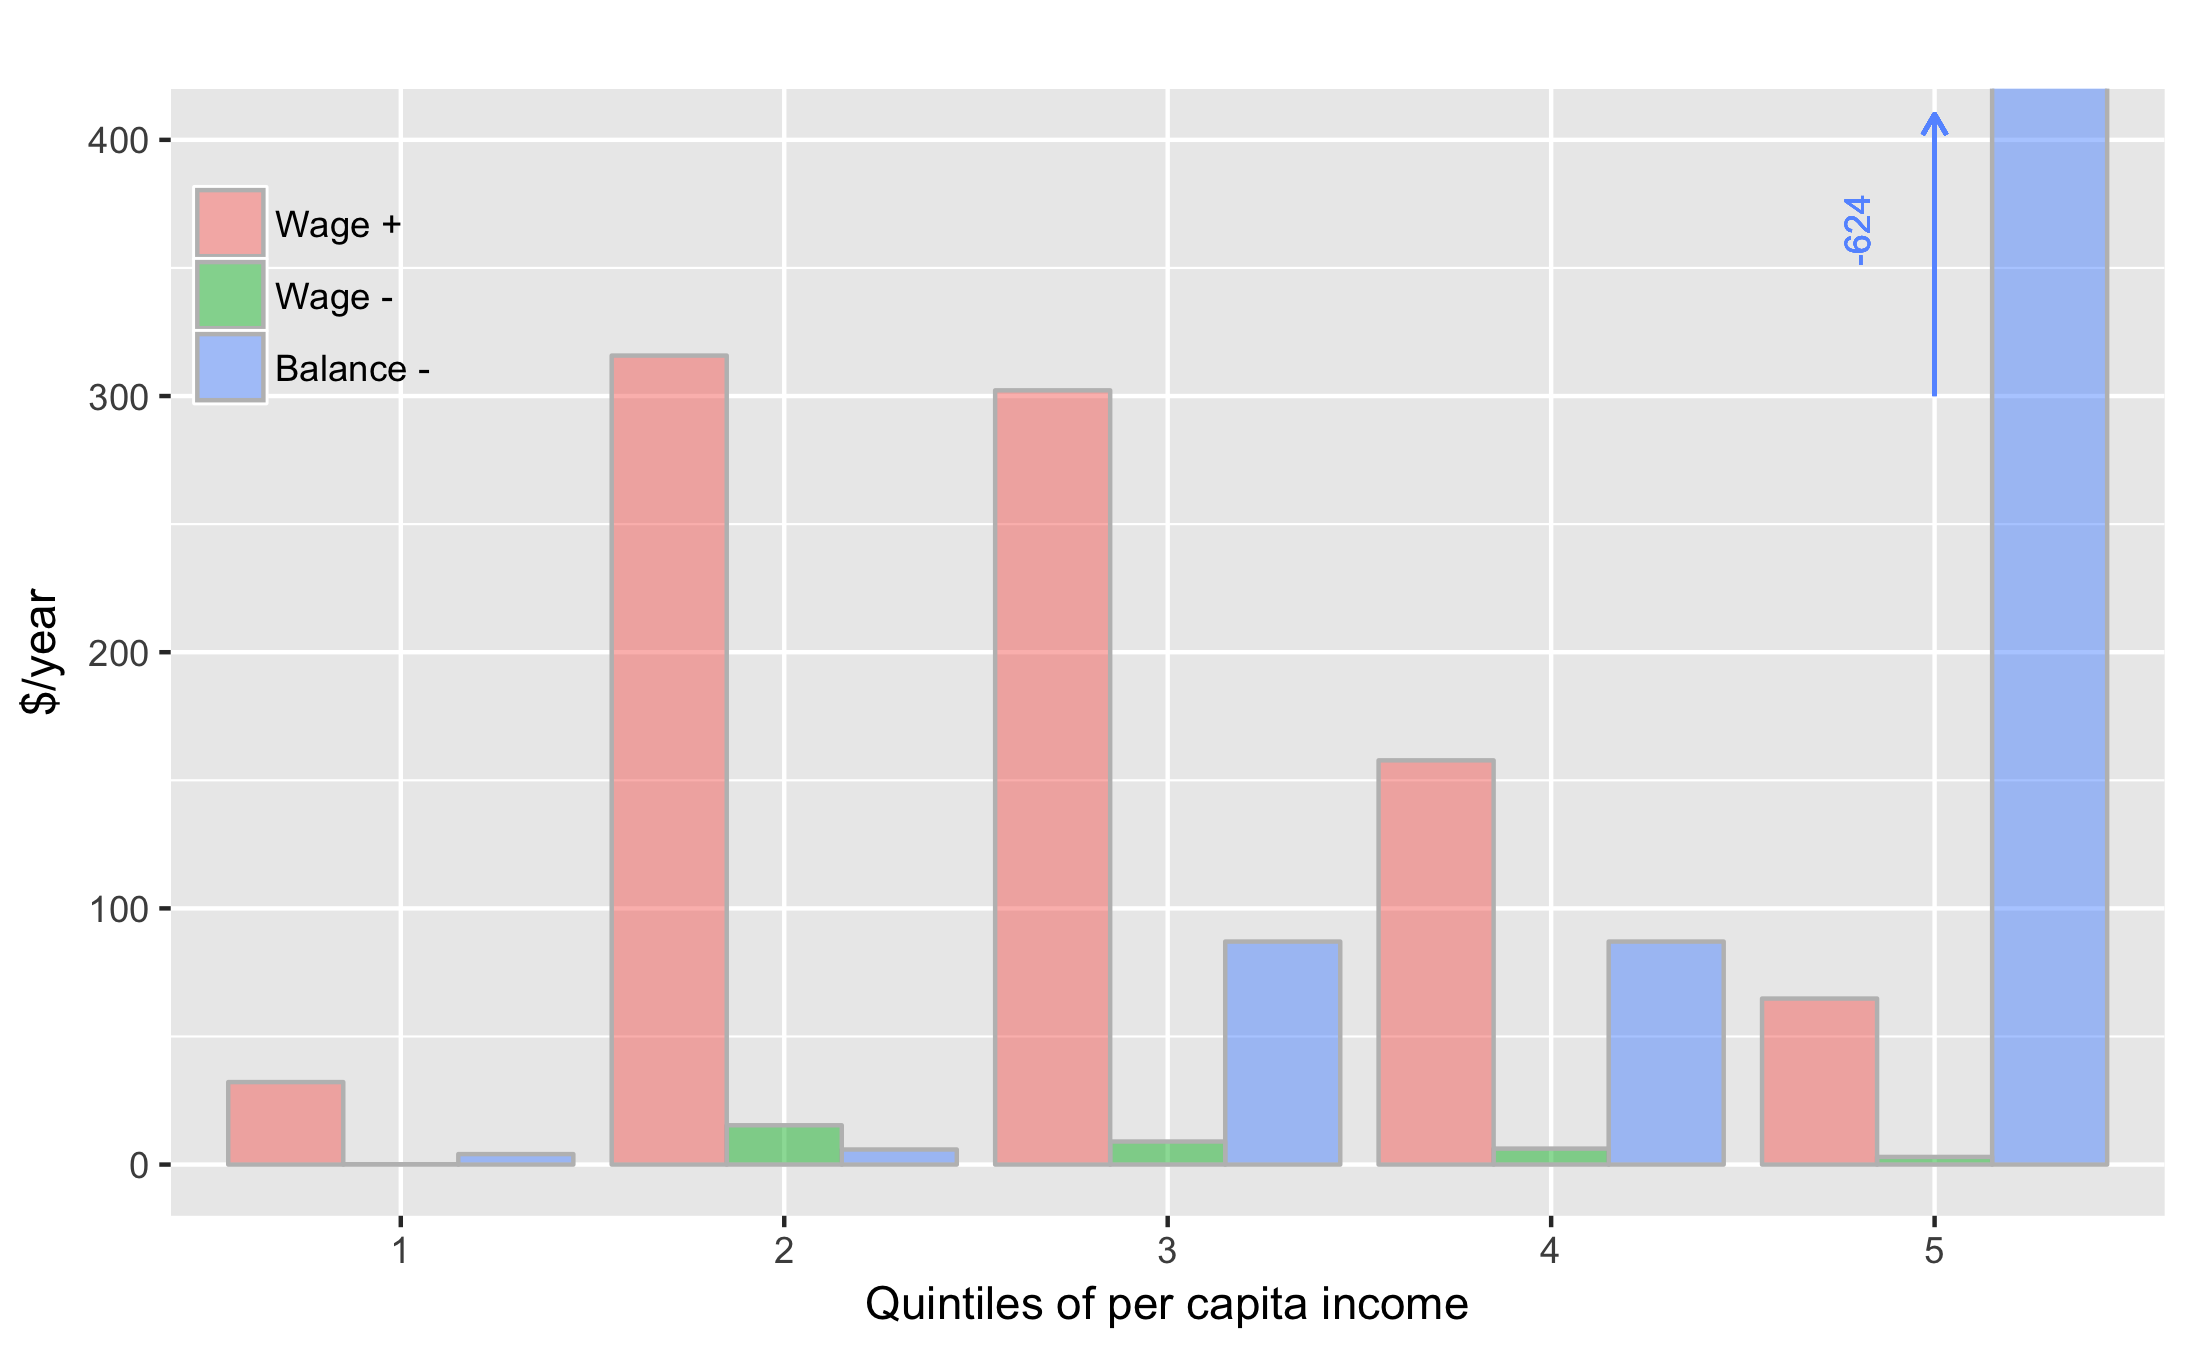
\includegraphics[scale = 0.13]{../Images/policy_est_eta001}
\caption{From $\eta^{teens}_{lit} = - 0.1$ to  $\eta^{teens}_{lit} = - 0.01(\Delta^{-}90\%)$}
\end{figure}	
\end{frame}

\begin{frame}[noframenumbering]{Sensitivity Analysis: Status Quo}
\begin{figure}[h!]
\centering
\hspace*{-3em}
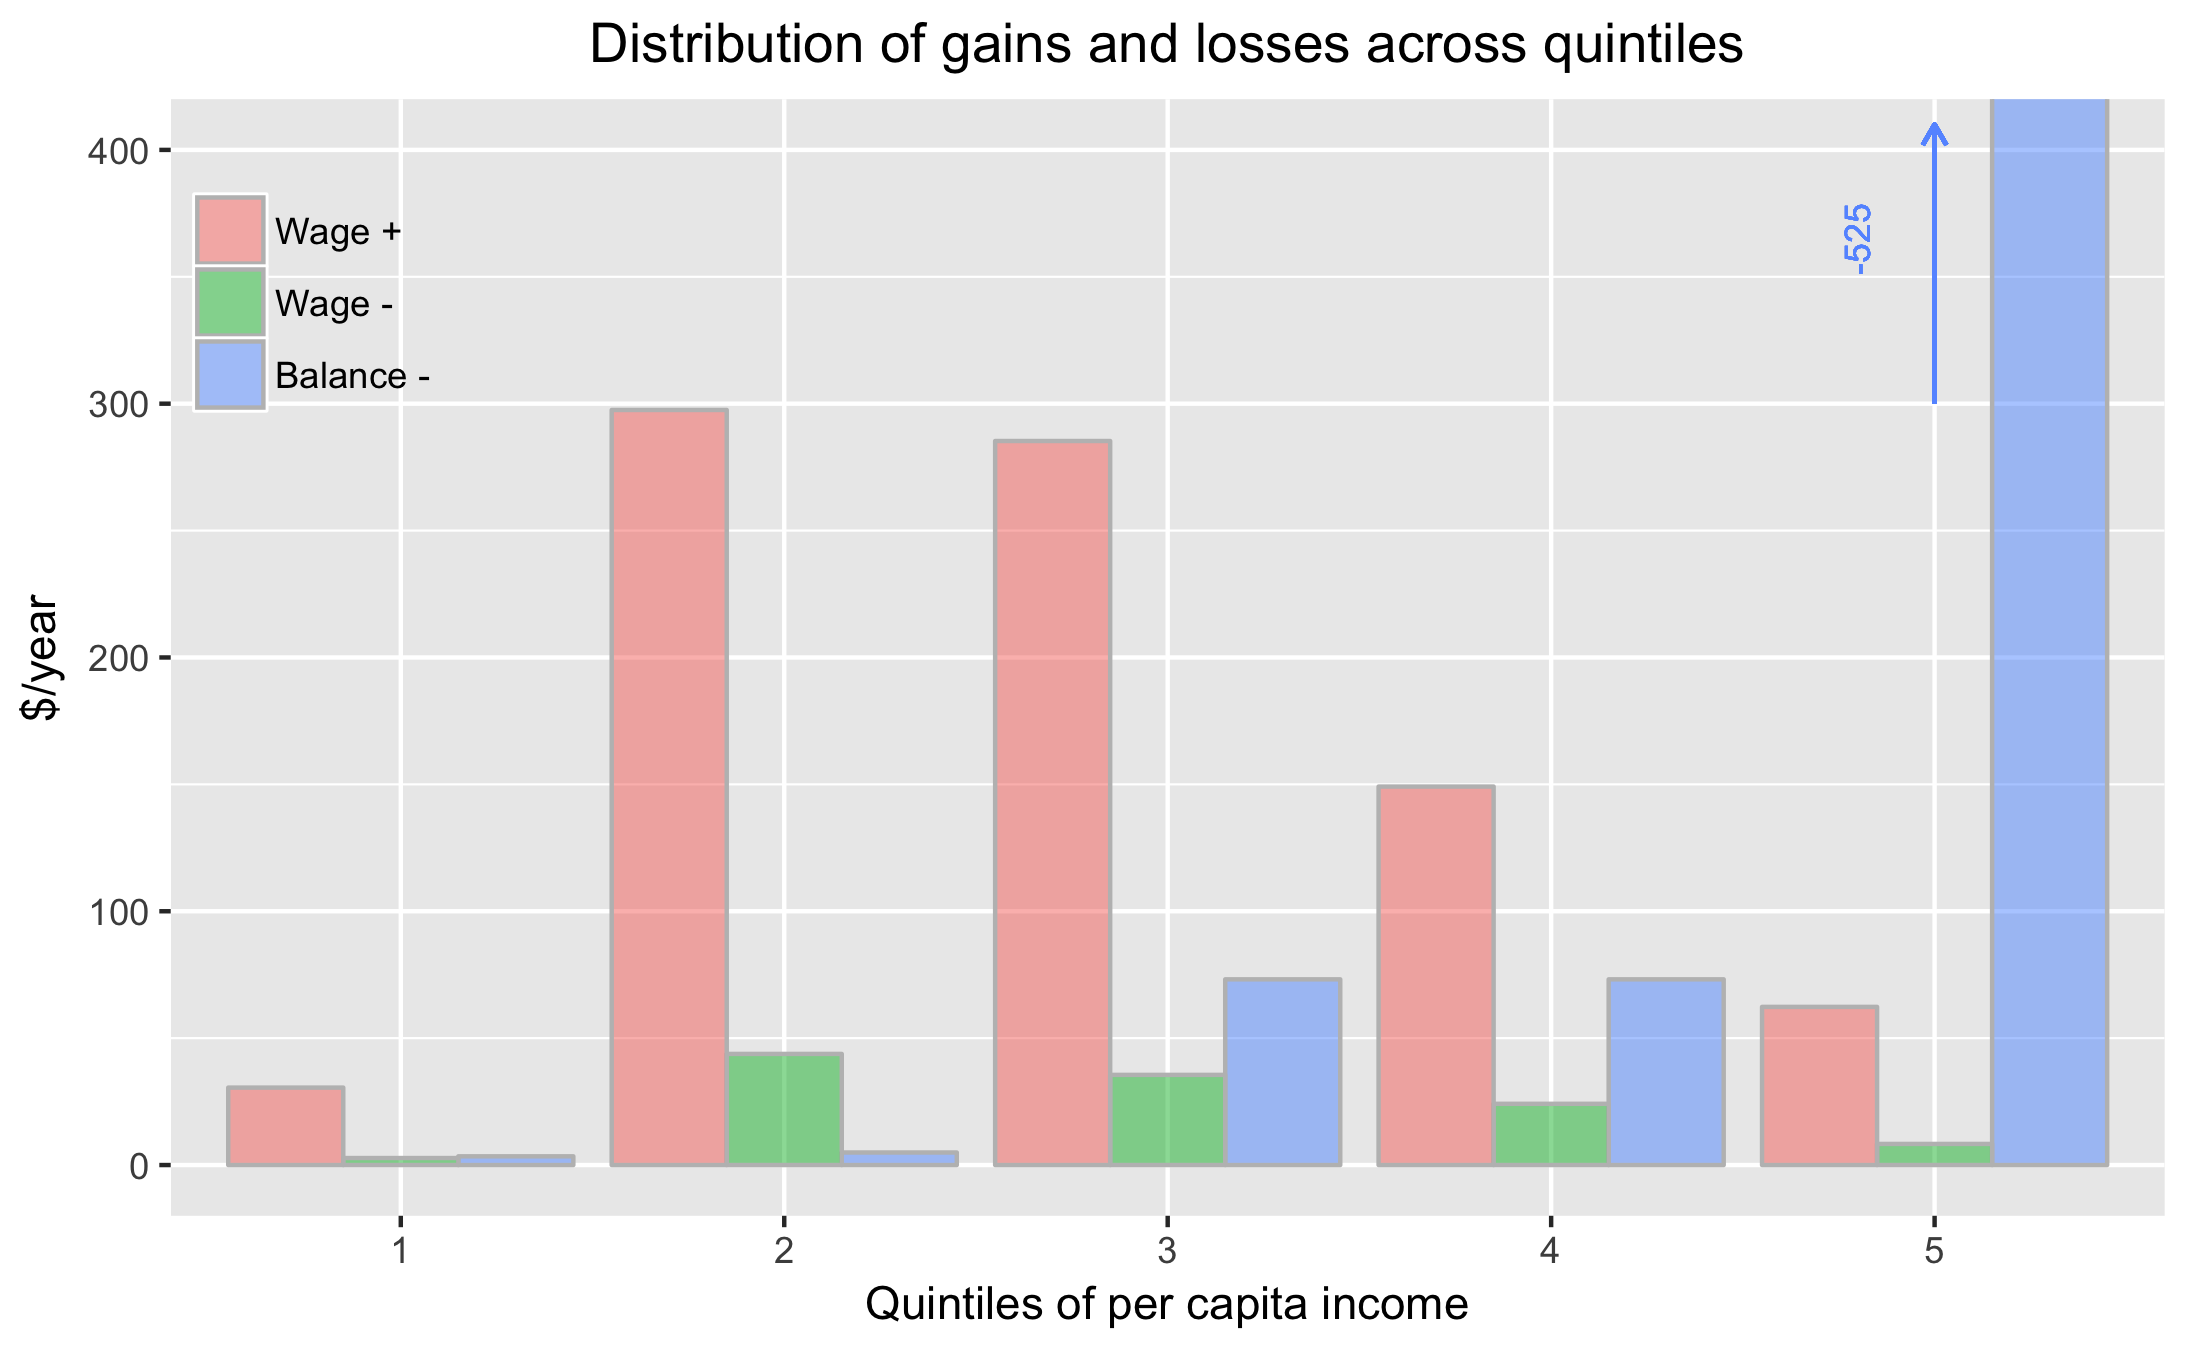
\includegraphics[scale = 0.13]{../Images/policy_est}
\caption{Default settings {\white $ \eta $} }
\end{figure}	
\end{frame}

\begin{frame}{SA: Change in Distribution of Balance Loses}
\begin{figure}[h!]
\centering
\hspace*{-3em}
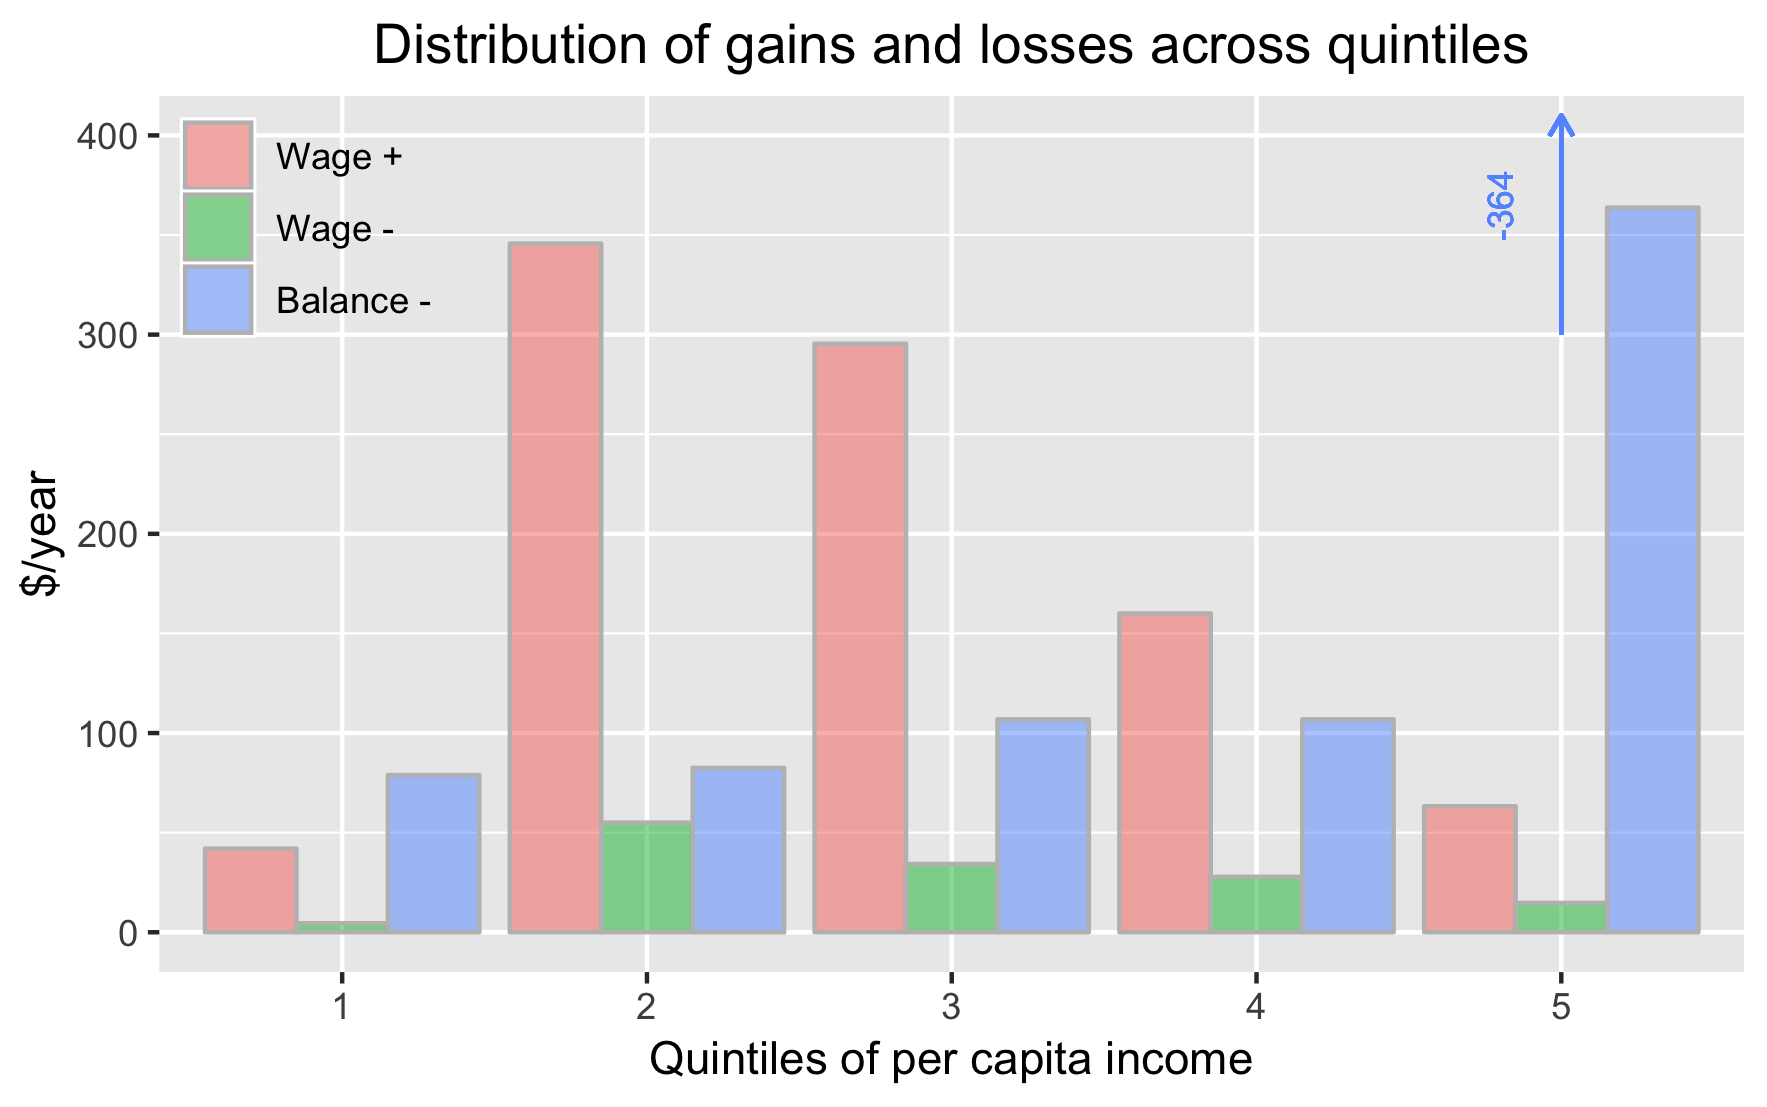
\includegraphics[scale = 0.13]{../Images/policy_est_bl_204040}
\caption{From $(1PL, 6PL) \sim (1\%, 29\%, 70\%)$ to  $(20\%, 40\%, 40\%)$}
\end{figure}	
\end{frame}


\begin{frame}{Sensitivity Analysis For Multiple Parameters}
\vspace*{-1.2em}
\begin{table}
\caption{$\%\Delta W$ for a $\%\Delta$ in inputs. Two sample policy makers.}
\scalebox{0.7}{
\begin{tabular}{ll|c|c|c|c}
\hline
	   &						 & \multicolumn{4}{|c}{Re-distributional Preferences} \\
	   &						 & \multicolumn{2}{|c|}{Dislikes $(\rho = -0.1)$} & \multicolumn{2}{|c}{Likes $(\rho = 0.1)$} \\ \hline
Source & Input                & $10\% \Delta^{+}$ 	& $10\% \Delta^{-}$ & $10\% \Delta^{+}$ 	& $10\% \Delta^{-}$\\ \hline
\multicolumn{2}{l|}{Data}     &        &             		&  	\\
	& Annual wage growth ($g_{w}$)  	&	-3\% 	& 2\% 		&	-2\% 	& 1\%		\\
	& Annual growth in $N$ 			&	0.8\% 	& -0.9\%	 	&	0.5\% 	& -0.5\%	 \\
\multicolumn{2}{l|}{Research}        &        	&      	 	&	\\
    & $\eta_{teen}$     				&  -4\%    	&  4\%      &  -2\%    	&  2\%	    \\
   	& Ripple Scope $(8.7, 11.5)$     &  37\%    	&  -24\%    &  21\%    &  -14\%	    \\
   	& Ripple Intensity $(50\% \Delta w)$& 5\%     &  -5\%     &  3\%     &  -3\%	   \\
\multicolumn{2}{l|}{Guess Work}      &        	&          	&           \\
   	& Extrapolation factor ($F_{ex}$)&  -3\%    	&  2\%    	&  -1\%    &  1\%	    \\ 
   	& Non compliance ($\alpha_{1}$)  &  -7\%    	&  7\%      &  -4\%    &  4\%	    \\
   	& Substitution factor ($F_{sub}$)&      		&  20\%     &     		&  -8\%	    \\ 
   	& Net benefits					&    -5\%  	&  5\%      &     2\%  	&  -2\%	    \\
   	& Distribution of balance losses  &   \multicolumn{2}{c|}{}&    \multicolumn{2}{c}{} \\
    & Current: $(1\%, 29\%, 70\%)$	& 	\multicolumn{2}{c|}{} &   \multicolumn{2}{c}{}\\
	& 	 $(1\%, 4\%, 95\%)$			&    \multicolumn{2}{c|}{22\%}     &    \multicolumn{2}{c}{13\%} 	    \\	 
  	& 	 $(5\%, 35\%, 60\%)$			&    \multicolumn{2}{c|}{-17\%}     &    \multicolumn{2}{c}{-9\%} 	    \\
  	& 	$1/N$						&    \multicolumn{2}{c|}{-129\%}     &    \multicolumn{2}{c}{-73\%}	   \\
\end{tabular}
}
\end{table}
\end{frame}

\section[Discussion]{Discussion}
% 5mins
\setbeamercovered{transparent}

\begin{frame}{Limitations}
\begin{itemize}
\item There is additional scope for reproducibility.
\item Complete case study requires extensive institutional knowledge.
\item Guidelines need to be build based on consensus of practitioners. 
\end{itemize} 
\end{frame}

\begin{frame}{Discussion}
\onslide<1>{
Let's assume this becomes the new status quo. 
\begin{itemize}
\item Costs of producing the next report on effects of minimum wage will be very small. 
\item Every additional effort will imply improvements on the ``state of the art'' report (e. g. $dBL$; $\eta(MW), \alpha_{1}(MW)$)
\item Learning about one parameter (QALYs, DWL) will update estimates \textit{across} reports.  
\item Much easier to have a substantive and normative policy debate. Pilot example: {\blue\texttt{\href{https://fhoces.shinyapps.io/example_min_wage/}{\underline{Shiny App!}}}}.
} 
%\onslide<2>{
%\item Two type of contributions ($\sim$software development):
%	\begin{itemize}
%	\item Short term: Within a given time period the model should be taken as given. Less freedom, but direct impact on the policy analysis. 
%	\item Long term: Structural revisions occur in parallel and are incorporated in future cycles of the analysis.
%	 	\end{itemize}
%}
%\onslide<2>{
%\item Who should work on this:
%\begin{itemize}
%\item Analytic reviewers of report; Research division within agencies; Study Commissions (``MWSC or MSWC?'' %\citep{card2016interview})
%\item Public policy schools. 
%\item Think tanks; Bank of knowledge \citep{clemens2016new}.
%\end{itemize}
%\item Next Steps
%\begin{itemize}
%\item BG: Reproduce meta-analysis and simulate new types of evidence; Improve DD; Incorporate %comments (especially from CBO); Deploy online (open source); Write!
%\item AG: $dBL$; $\eta(MW), \alpha_{1}(MW)$ and others ; \texttt{\href{https://%fhoces.shinyapps.io/example_min_wage/}{Shiny App!}}
%\end{itemize}

%}
\end{itemize}
\end{frame}

\begin{frame}{BITSS/CEGA's next step to push OPA forward}
\begin{itemize}
\item Partner with key policy analysts to build more case studies (CBO, Tax policy/Inequality, Chilean pension reform)
\item Guidelines and trainings
\item Developing a new model for collaboration among policy analysts, policy-makers and researchers, with the aim of fostering more direct impact on high-level government decisions
\end{itemize}
\end{frame}

\begin{frame}{Your next steps to push OPA forward}
\begin{itemize}
\item Collaborate with BITSS to open up your PA. 
\item Fund OPA: directly or conditionally.
\item Train students/analysts in OPA.
\item Present/showcase your OPA. Pioneers: GiveWell, AEI.  
\item Nominate a PA to be open. 
\end{itemize}
\end{frame}

\begin{frame}{An Aspiration}
   \begin{tikzpicture}[remember picture,overlay]
       \node[at=(current page.center), xshift =0em, yshift = -1.4em] {
         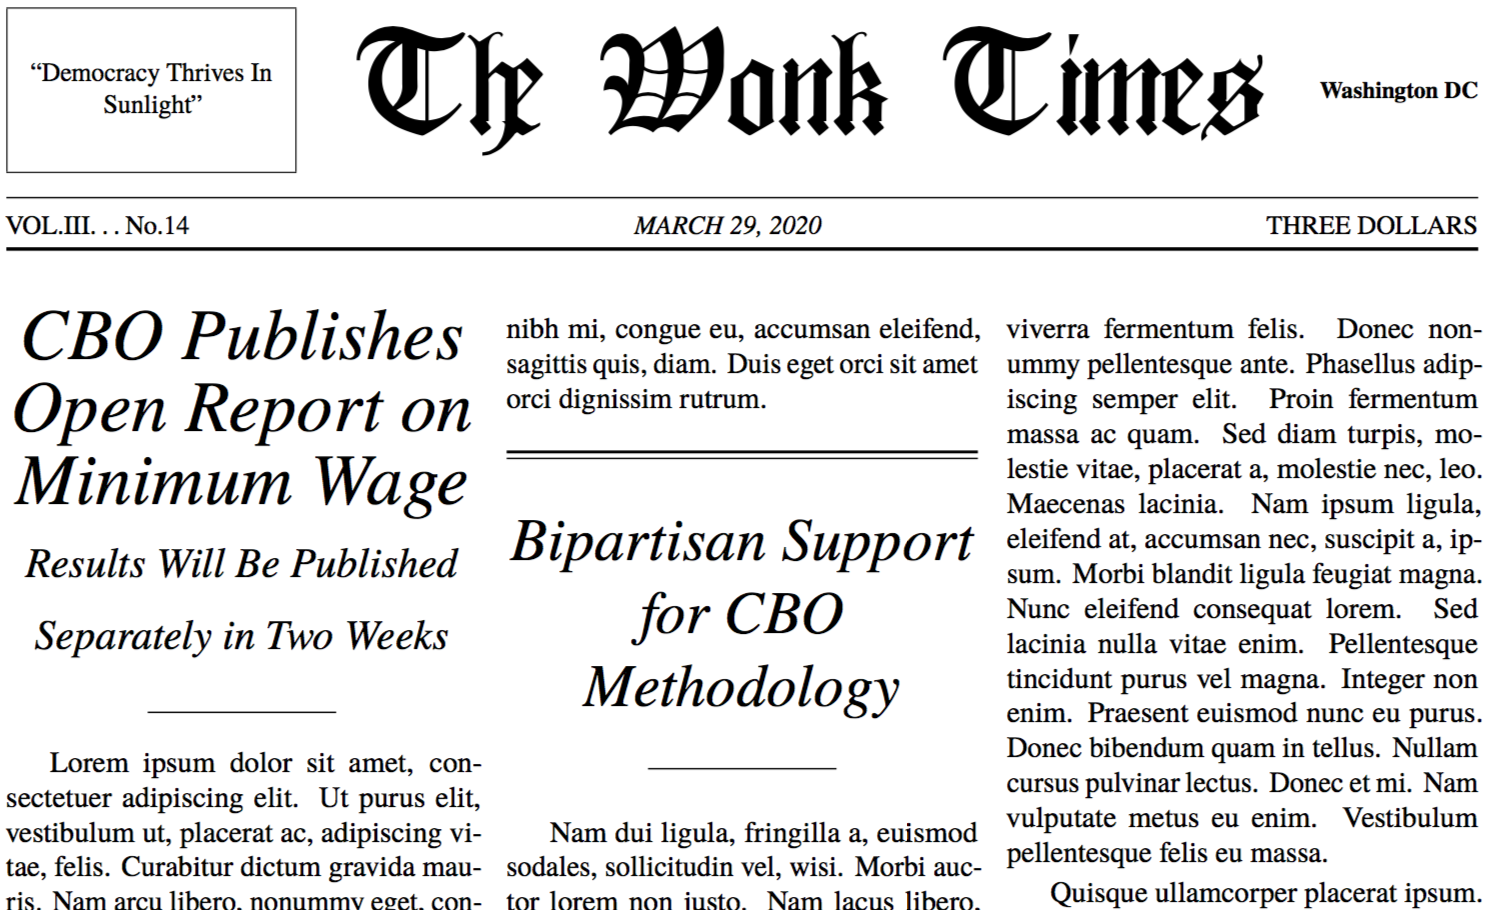
\includegraphics[width=.98\paperwidth]{../Images/aspiration.PNG}
       };
   \end{tikzpicture}
\end{frame}



\begin{frame}[noframenumbering]
\begin{center}
\vspace*{6em}
{\LARGE Thank you.\\}
\bigskip
{\small
Pre-prints:\\
{\blue \href{https://osf.io/preprints/bitss/jnyqh}{Why OPA} } \\
{\blue \href{https://osf.io/preprints/bitss/ba7tr/}{OPA Case Study}  } \\
\medskip
Slides at \\
{\blue \href{http://www.github.com/fhoces/CBO2018}{github.com/fhoces/CBO2018}  }
\bigskip \\
\href{mailto:fhoces@berkeley.edu}{fhoces@berkeley.edu}
}
\end{center}
\end{frame}

\appendix

\begin{frame}[noframenumbering]
\begin{center}
Back-up slides
\end{center}
\end{frame}








\backupbegin



\begin{frame}[label=before]{Easier Methodological Appraisal. Example: dis-employment effects \textbf{Before}}


Steps taken to verify the analysis \&  employment variation $(\widehat{\Delta E}\times 1000)$ at each line\footnotemark 

\footnotetext[1]{Assuming target population $\approx 22$ million, $\overline{\Delta w_{w\leq MW^{'}}} \approx 14\%$, and non-compliance $\approx 15\%$ }
 

\begin{enumerate}
\pause
\item Find an elasticity: -0.1 (page 25): {\red $\widehat{\Delta E} \approx 300$ }
\pause
\item What about adults? $\eta^{adults}=\frac{1}{3}\eta^{teens}$ (page 28):  {\red $\widehat{\Delta E} \approx 100$  } 
\pause
\item What about the adjustment? $\widetilde{ \eta^{g}_{w\leq MW} } =  \frac{\eta^{g}_{lit}}{p^{g}_{w\leq MW}} \times \frac{\%\Delta MW}{\overline{\%\Delta w^{g}}}$ (page 26-28 + 2 papers):   {\red $\widehat{\Delta E} \approx 1,100$  } 
\pause
\item The adjustment factors $\frac{1}{p^{g}_{w\leq MW}} \times \frac{\%\Delta MW}{\overline{\%\Delta w^{g}}} = F^{g}_{adj}$ are not computed from the data (3.2 teens, 19.5 adults). Instead: $F^{teen}_{adj} = F^{adult}_{adj}= 4.5$ (page 28) ${\red\widehat{\Delta E} \approx 500}$   
\end{enumerate}
\textit{Steps 2-4 took several days of work! }
\small{\hyperlink{map_cbo}{\beamerbutton{}}}
\end{frame}

\begin{frame}[label=equations]{{\small\hyperlink{map_cbo}{\beamerbutton{}}}Equations from Model in DD}
\subsection{Employment}

\begin{flalign}\label{N_final}
\widehat{\Delta E} &= N \times \eta \times \% \Delta w  + \text{Other factors} &&
\end{flalign}

\begin{flalign}
\widehat{ N^{s}_{final} } &= \hat{ g_{N}(t'|t) } \times  \hat{ N^{s}_{t} }  \times P(\hat{w'} \leq MW^{new}|s)  \times (1 - \hat{ \alpha^{s}_{1} } - \hat{ \alpha^{s}_{2} })  \hspace{2em} s = \{teens, \, adults \} &&
\end{flalign}

The elasticity for adults from the literature is define as the one for teenagers with an extrapolation factor. 
  
\begin{flalign}
\eta^{adults}_{lit} &= \eta^{teens}_{lit} \times F_{extrapolation}&& 
\end{flalign}
\end{frame}

\begin{frame}{{\small\hyperlink{map_cbo}{\beamerbutton{}}}Adjustments to the elasticity of labor demand}
Following Neumark and Wascher (2008),  Brown (1999). First:

\begin{flalign}
\eta^{s}_{lit} &= p^{s}_{w\leq MW} \eta^{s}_{w\leq MW} + (1 - p^{s}_{w\leq MW})\eta^{s}_{w > MW}  \hspace{2em} s = \{teens, \, adults \} &&\nonumber 
\end{flalign}

Second, assume $\eta^{s}_{w\leq MW} = 0$:

\begin{flalign}
\eta^{s}_{w\leq MW} &= \frac{\eta^{s}_{lit}}{p^{s}_{w\leq MW}}  \hspace{2em} s = \{teens, \, adults \}&& \nonumber
\end{flalign}

And third, adjust for the effective average wage variation for each group ($\overline{\%\Delta w^{s}}$):

\begin{flalign}\label{eta_final}
\widetilde{ \eta^{s}_{w\leq MW} } &=  \frac{\eta^{s}_{lit}}{p^{s}_{w\leq MW}} \times \frac{\%\Delta MW}{\overline{\%\Delta w^{s}}} = \eta^{s}_{lit} \times F^{s}_{adjs}  \hspace{2em} s = \{teens, \, adults \}&&
\end{flalign}

\end{frame}


\begin{frame}{{\small\hyperlink{map_cbo}{\beamerbutton{}}}Final Effect on Employment}

\begin{flalign}
 \widehat{ \Delta E } &= \sum_{g\in\{A,T\}} \left( \widehat{ N^{final}_{g} } \times \widetilde{ \eta^{g}_{w\leq MW} }\times \overline{\%\Delta w^{g}}  \right) - \widehat{OF}&&
\end{flalign}
\end{frame}

\begin{frame}{{\small\hyperlink{map_cbo}{\beamerbutton{}}}Effect on Wages}
\subsection{Wages}  

\begin{flalign}\label{no_comp}
w^{''} &=
\begin{cases}
w' \quad if \quad  w \in U[0,1]<\alpha_1 \\
w^{new} \quad \quad o/w
\end{cases} &&
\end{flalign}

\begin{flalign}
w^{new} &=
\begin{cases}
w'/2 \quad if \quad  w \in U[0,1]<\alpha_{aux} \\
\widetilde{w^{new}} \quad \quad o/w
\end{cases} &&
\end{flalign}

Ripple Effects

\begin{flalign}\label{ripple_wages}
\widetilde{w^{new}}  &=
\begin{cases}
MW' \quad if \quad  w' < R_{lb} \\
MW' + R^{I}(w' - R^{s}_{lb} )\quad if \quad  w' \in [R_{lb}, MW') \\
w' + R^{I}(R^{s}_{ub} - w' )\quad if \quad  w' \in [MW', R_{ub}) \\
w' \quad \quad o/w
\end{cases} &&
\end{flalign}
\end{frame}

\begin{frame}{{\small\hyperlink{map_cbo}{\beamerbutton{}}}Computing Income}
\vspace{-0.5em}
\subsection{Income}

\begin{flalign}
 y'_{i,h} &= \sum_{i\in N_{h}} \left( g_{nw}(t'|t) nw_{i} + w'_{i}  \right)/N_{h} &&\nonumber \\
 y''_{i,h} &= \sum_{i\in N_{h}} \left( g_{nw}(t'|t) nw_{i} + w''_{i}  \right)/N_{h} &&
\end{flalign}

\textbf{Final Policy Estimates}
\vspace{-0.5em}
\begin{flalign}
 WG_{i} &=  \left(y''_{i}  - y'_{i} \right) \mathbf{I}\left(y''_{i}  > y'_{i} \right)  &&\\
 WL_{i} &=  \left(y'_{i}  - y"'_{i} \right) \mathbf{I}\left(y''_{i}  < y'_{i} \right)  && \\
 BL &= \sum_{i} WG_{i} - F_{sub} \sum_{i} WL_{i};\quad 
 BL_i = BL \times dBL &&\\
 \overline{WG_{Q}} &= \frac{\sum_{i \in Q} WG_{i}}{N_{pop}/5} \quad
 \overline{WL_{Q}} = \frac{\sum_{i \in Q} WL_{i}}{N_{pop}/5}  && \nonumber\\ 
 \overline{BL_{Q}} &= \frac{\sum_{i \in Q} BL_{i}}{N_{pop}/5} &&\label{last.eq}  
\end{flalign}

\end{frame}


\begin{frame}[plain, label=no_inet]{Snapshots of DD}
\vspace{-2em}
\begin{figure}[h!]
\centering
\hspace{-5em} 
\includegraphics[scale = 0.28]{../Images/Screen_Shot1}
\hyperlink{demo}{\beamerbutton{}}
\end{figure}	

\end{frame}

\begin{frame}[plain]{Snapshots of DD\hyperlink{demo}{\beamerbutton{}}}
\vspace{-2em}
\begin{figure}[h!]
\centering
\hspace{-5em} 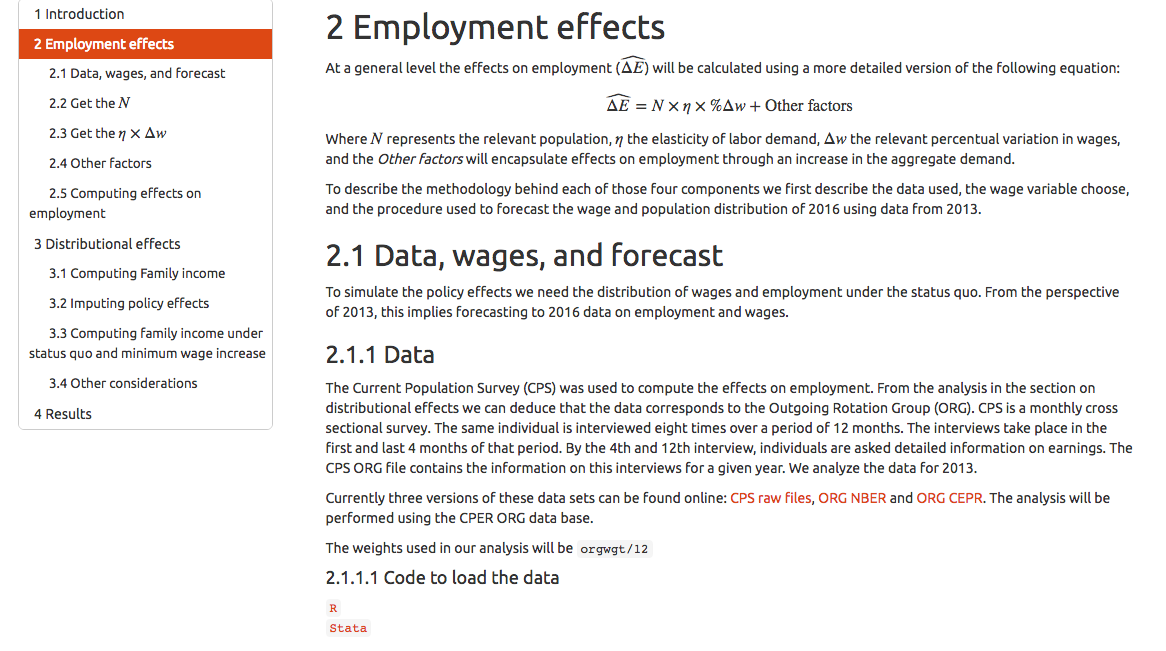
\includegraphics[scale = 0.28]{../Images/Screen_Shot2}
\hyperlink{demo}{\beamerbutton{}}
\end{figure}	
\end{frame}

\begin{frame}[plain]{Snapshots of DD\hyperlink{demo}{\beamerbutton{}}}
\vspace{-2em}
\begin{figure}[h!]
\centering
\hspace{-5em} 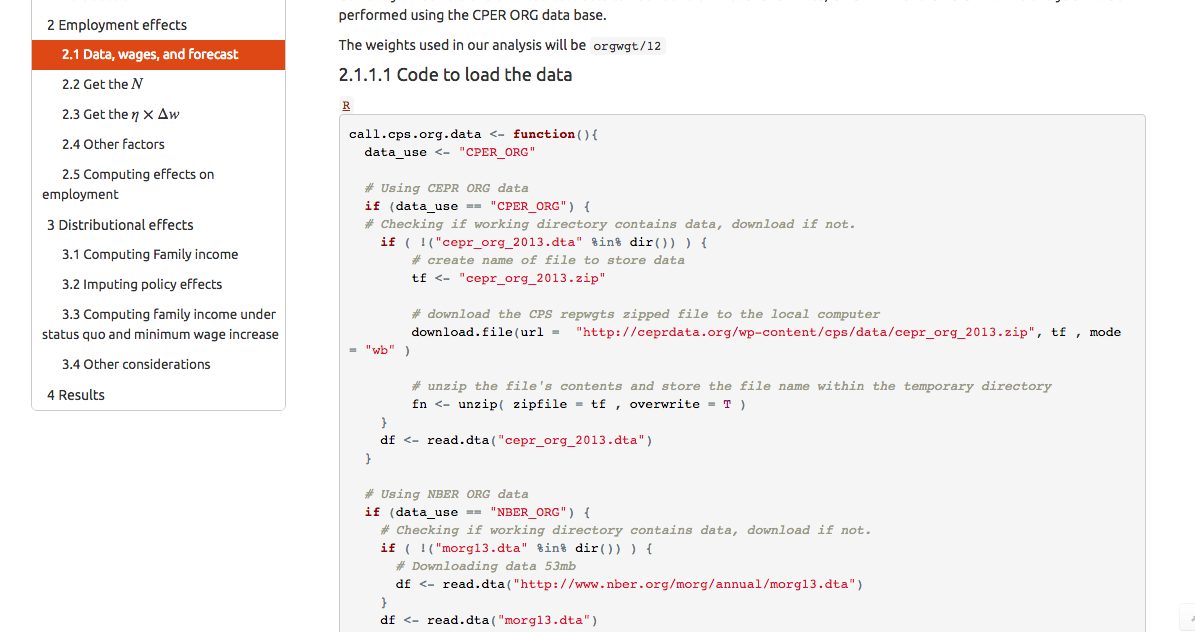
\includegraphics[scale = 0.28]{../Images/Screen_Shot3}
\hyperlink{demo}{\beamerbutton{}}
\end{figure}	
\end{frame}

\begin{frame}[plain]{Snapshots of DD\hyperlink{demo}{\beamerbutton{}}}
\vspace{-2em}
\begin{figure}[h!]
\centering
\hspace{-5em} 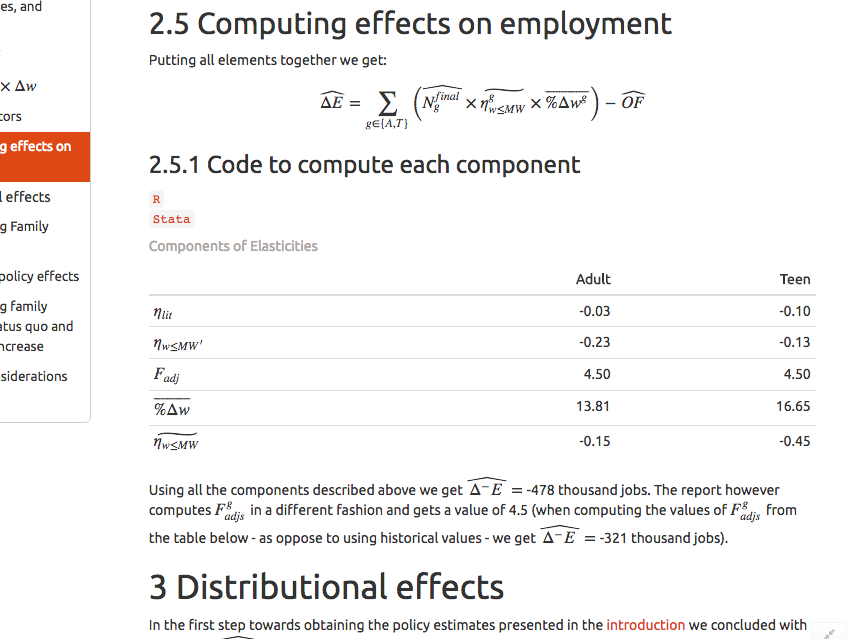
\includegraphics[scale = 0.28]{../Images/Screen_Shot4}
\hyperlink{demo}{\beamerbutton{}}
\end{figure}	
\end{frame}

\begin{frame}[plain]{Snapshots of DD\hyperlink{demo}{\beamerbutton{}}}
\vspace{-2em}
\begin{figure}[h!]
\centering
\hspace{-5em} 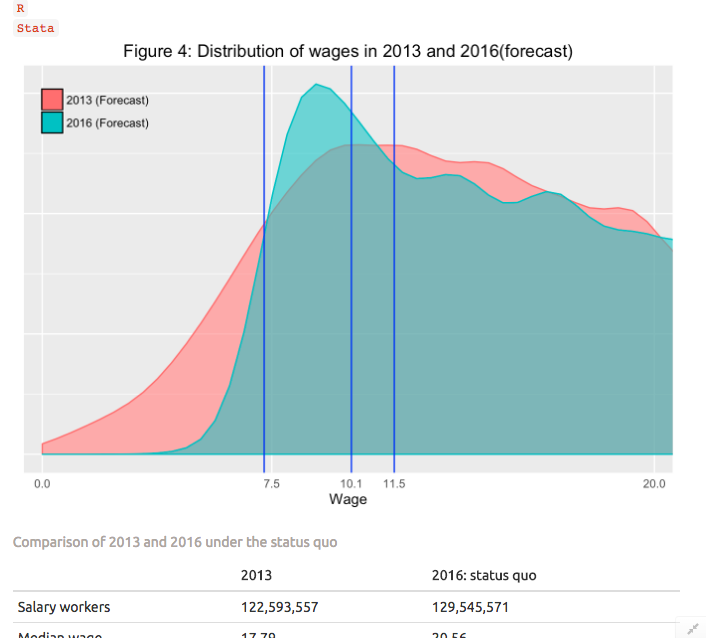
\includegraphics[scale = 0.28]{../Images/Screen_Shot5}
\hyperlink{demo}{\beamerbutton{}}
\end{figure}	
\end{frame}

\begin{frame}[plain]{Snapshots of DD}
\vspace{-2em}
\begin{figure}[h!]
\centering
\hspace{-5em} 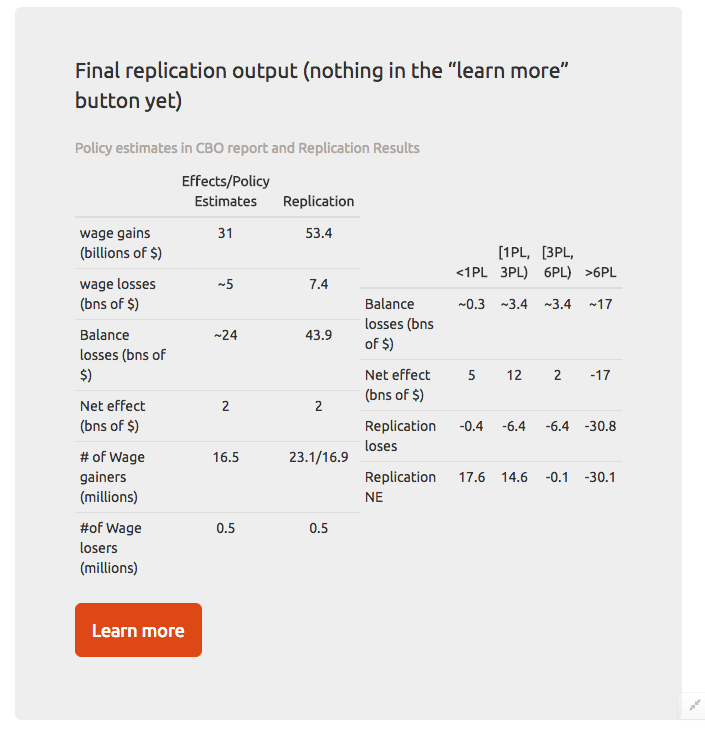
\includegraphics[scale = 0.28]{../Images/Screen_Shot6}
\hyperlink{demo}{\beamerbutton{}}
\end{figure}	
\end{frame}



\begin{frame}[label=full_model]{Clear connection between sources and inputs}
\centering
\resizebox{25em}{11em}{%
\begin{tabular}{P{1em}P{16em}|P{25em}}
\hline
\multicolumn{2}{c|}{Source} & \multicolumn{1}{c}{Input} \\ \hline
\multicolumn{2}{l|}{\textit{Data}} &  \\
 & CPS ORG 2013 \linebreak (CEPR version) & Number of salary workers in 2013 $(\widehat{ N^{g}_{final} } \quad g\in\{teen, adult\} )$; Fraction of workers below the new minimum wage $(P_{\hat{w} \leq MW^{1}|g})$; Average wage variation for those below the new min wage $(\overline{\%\Delta w^{g}})$; Non-compliance rate $(\alpha_{1}^{g})$\\
  &  &  \\ 
 & CPS ASEC 2012 \linebreak (CEPR version) & Wages and Non-Wage Income distribution $(dF_{w}, dF_{nw})$; Household size ($N_{h}$); Hours/weeks worked $(\hat{w} , \hat{h})$\\
 & State level Min. Wage (DOL) & Trends in state min. wage $(MW^{s}_{t})$ \\
 & 10-year economic forecast (CBO) & Predicted worker growth by 2016 (in 2013) $(\hat{g_{N}})$; Wage growth in by 2016 $(\hat{g_{w}})$; Non-wage growth by 2016 $(\hat{g_{nw}})$ \\
 &  &  \\ \hline
\multicolumn{2}{l|}{\textit{Research}} &  \\
  & Elasticity of labor demand for teenagers &  $\eta_{teen}^{lit} = -0.1$ \\
 & Ripple effects & From $R_{lb} = \$8.7$ to $R_{ub} = \$11.5$ with a ``ripple'' intensity of $R_{I} = 50\%$  \\
 &  &  \\ \hline
\multicolumn{2}{l|}{\textit{Guess Work}} &  \\
 & Extrapolation factor from teenagers to adults  &  $F_{ex} = 1/3$ \\
 & Net benefits &  $\hat{NB} = \$2 billion$  \\
  & Adjustment to account for effective wage variation and affected population &  $F_{adj} = 4.5$  \\
 & Aggregate consumption effects on employment &  $\hat{OF} = 40,000 \, new \, jobs$\\
 & Distribution of balance loses & $dBL = (1\%, 29\%, 70\%)$  if income $\in [0, 1PL, 6PL, + )$  \\
 & Fract. of wage loses used to pay wage gains &  $F_{subs} = 1$ \\
 & Job killing process: fraction of jobs & Cut wages in half for twice the number of jobs destroyed \\ \hline
\end{tabular}}

\end{frame}


\begin{frame}{Fully specified model}
\centering
\resizebox{25em}{9em}{%
\begin{tabular}{P{19em}|P{9em}}
\hline
\multicolumn{1}{c|}{Model} & {\centering Policy estimate \linebreak (per quintile) } \\ \hline
Predicted household income with and without min wage increase. \linebreak \textbf{Depends on}: $\widehat{ N^{g}_{final} },  P_{\hat{w} \leq MW^{1}|g}, \overline{\%\Delta w^{g}},\alpha_{1}^{g},$ $dF_{w}, dF_{nw}, N_{h}, \hat{w}, \hat{h}, MW^{s}_{t}, \hat{g_{N}}, \hat{g_{w}},\hat{g_{nw}},$ $\eta_{teen}^{lit}, R_{lb}, R_{ub}, R_{I}, F_{ex}, F_{adj}, \hat{OF}$  &  Average gain in per capita income due to net wage increase. \linebreak ($\overline{WG_{q}}$) \\
\hline
%\small{\hyperlink{wage_gain}{\beamerbutton{}}}

Predicted household income with and without min wage increase. \linebreak \textbf{Depends on}: $\widehat{ N^{g}_{final} },  P_{\hat{w} \leq MW^{1}|g}, \overline{\%\Delta w^{g}},\alpha_{1}^{g},$ $dF_{w}, dF_{nw}, N_{h}, \hat{w}, \hat{h}, MW^{s}_{t}, \hat{g_{N}}, \hat{g_{w}},\hat{g_{nw}},$ $\eta_{teen}^{lit}, F_{ex}, F_{adj}, \hat{OF}$  &  Average loss in per capita income due to net wage decrease. \linebreak ($\overline{WL_{q}}$) \\
\hline
%\small{\hyperlink{wage_loss}{\beamerbutton{}}}
Distribution of balance loses \linebreak \textbf{Depends on}: $\overline{WG_{q}}(\cdot), \overline{WL_{q}}(\cdot), \hat{NB},$ $F_{subs}, dBL$  &  Average loss in per capita income to balance wage gains. \linebreak ($\overline{BL_{q}}$) \\
\hline\hline
{ \raggedright {\small \hyperlink{equations}{Equations}; \hyperlink{map_cbo}{Back} } }
\end{tabular}}

\end{frame}

\begin{frame}{Comparing the Trade-offs: A Toy Example}

Model for the normative comparison made by a policy maker (welfare function):

\begin{align*}
W(\rho) &= \sum_{i \in N} \left( \omega_{wg}  wg_{i} + \omega_{wl} wl_{i} + \omega_{bl} bl_{i} \right) \omega^{d}_{i}(Q_{i}, \rho) \\
\text{with:}& \nonumber \\
\omega^{d}_{i}(Q_{i}, \rho) &= \frac{(1 - \rho(Q_{i} - Q_{median}) ) }{\sum_{i} \omega^{d}_{i}(Q_{i}) } Q_{max} \quad \text{for }  \rho \in \left(-\frac{1}{2}, \frac{1}{2} \right) \nonumber
\end{align*}
$\rho>0$ represents positive valuation of progressive redistribution. $\rho<0$ represents positive valuation of regressive redistribution. 
\end{frame}


\begin{frame}{ Redistribiutional Preferences  \linebreak \vspace*{-1em} Toy Example ({ $\omega_{WG} = \omega_{WL} = \omega_{BL} = 1$}) }

\vspace{-.2em}
\begin{figure}[h!]
\centering
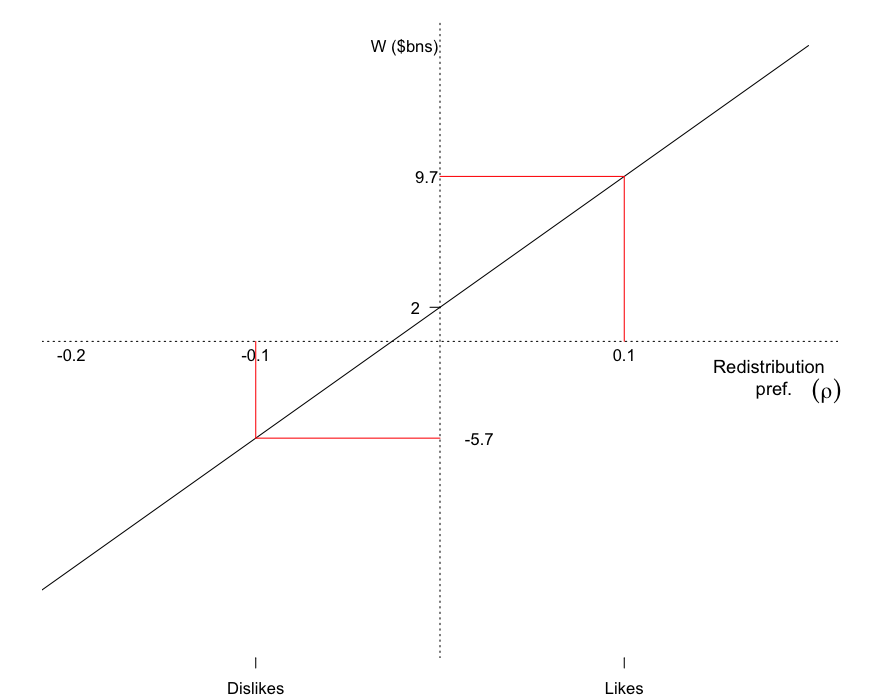
\includegraphics[scale = 0.35]{../Images/sample_pref}
\label{toy_ex}
\end{figure}	
\end{frame}


\begin{frame}{Motivation 2: An Academic Concern in 2013}
\begin{exampleblock}{}
  {\large ``I worry that someday sooner or later the existing social contract to take CBO scores at face value will break down. Conventional Certitudes that lack foundation cannot last indefinitely.''
}
  \vskip3mm
  \raggedleft{\small--- Charles Manski} \footnotesize{ \linebreak  Public Policy in an Uncertain World, 2013} 
  	  
\end{exampleblock}
\end{frame}

\begin{frame}{Motivation 2: A Reality In 2017}
   \begin{tikzpicture}[remember picture,overlay]
       \node[at=(current page.center), xshift = 2em, yshift = -1.4em] {
         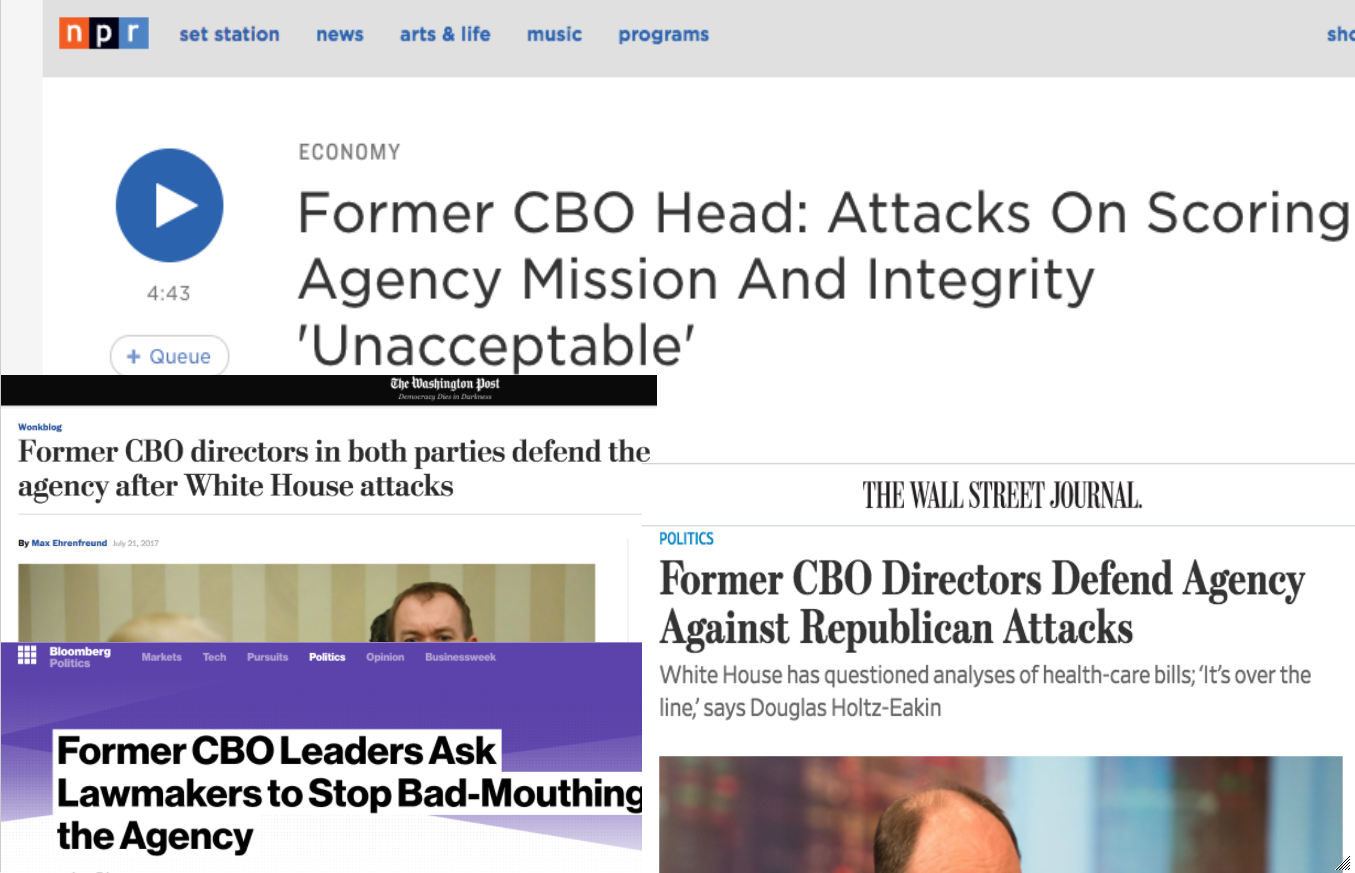
\includegraphics[width=.87\paperwidth]{../Images/CBO_under_attack.PNG}
       };
   \end{tikzpicture}
\end{frame}

  
\begin{frame}{Challenges And Suggestions}
\textbf{Challenges:}
\begin{itemize}
\item Policymakers may not want analyses to be open.
\item Analysts may wish to keep policy analyses ``closed''. 
\item For policy analysis contracted out to third parties: Opening methods will prevent them form reselling extensions.
\item  Initially reproducibility represents an additional layer of work.
\item Limits to sharing sensitivity of information, requires resources for adequate de-identification if open data is expected
\end{itemize}
\end{frame} 

\backupend




\end{document}

